% !TEX root = ./main.tex
% Thesis

% !TEX root = ./main.tex

\documentclass[11pt, oneside]{book}
\usepackage{times}
\usepackage{xstring}
\usepackage{ifthen}
\usepackage{graphicx}
\usepackage{microtype}
\usepackage{geometry}
\usepackage{lipsum}     % For placeholder text (ipsum)
\usepackage{array}
\usepackage{multirow}
\usepackage{longtable}
\usepackage{etoolbox}
\usepackage{fancyhdr}
\usepackage{arydshln}
\usepackage{indentfirst}    % Indent the first line everywhere in doc
\usepackage{setspace}
\usepackage{titlesec}
\usepackage[sorting=ydnt]{biblatex}
\usepackage{caption}
\usepackage{subcaption}
\usepackage{hyperref}   % Reference (for better navigation)
\usepackage{amssymb}
\usepackage{amsmath}
\usepackage{wasysym}
\usepackage{titletoc}
\usepackage{acronym}
\usepackage{xcolor}
\usepackage[color=red, linewidth=2bp]{pdfcomment}
\usepackage[capitalize]{cleveref}


% =========== Configurations ===========
% ------ Document formatting ------
% \setlength{\oddsidemargin}{0.125in}
% \setlength{\evensidemargin}{0.125in}
\geometry{
    a4paper,
    textwidth=6.25in,
    % textheight=8.7in,
    bottom=0.8in,
    top=1.5in,
    % lmargin=0.125in,
    % rmargin=0.125in,
}
% ------ Numbering and counters ------
% Section numbering depth
\setcounter{secnumdepth}{3}
% ------ Spacing ------
\onehalfspacing     % Text
\titlespacing{\section}{0in}{0.35in}{0.125in}
\titlespacing{\subsection}{0in}{0.35in}{0.125in}
% ------ Captions ------
\captionsetup{labelfont={bf}, labelsep={space}}
% ------ Graphics paths ------
\graphicspath{{figures/}}
% ------ Chapter font settings (Large and center titles) ------
\titleformat{\chapter}[display]
    {\normalfont\Large\centering\itshape}{Chapter \thechapter}{0.25in}
    {\normalfont\Large\centering\bfseries}
% \chapterfont{\Large\centering}
% ------ Table of contents ------
% TODO: The TOC titles should not be in bold and add heading
% \contentsmargin{2.55em}
% \dottedcontents{chapter}[0em]{\addvspace{0.5pc}}{1em}{0.5pc}
% ------ Clever Referencing ------
% \crefname{figure}{figure}{figures}
% ------ Bibliography ------
\addbibresource{Bibliography.bib}

% Macro definitions
% !TEX root = ./main.tex

% =========== Counters ===========
%%  magicrownumbers     Automatically set the row numbers in a table
%%                      context. Use '\rownumber' to put this in.
%%      Inspired from: https://tex.stackexchange.com/q/21243/253896
\newcounter{magicrownumbers}
\preto\tabular{\setcounter{magicrownumbers}{0}}
\newcommand{\rownumber}{
    \stepcounter{magicrownumbers}\arabic{magicrownumbers}
}

% =========== Macros ===========
%%  \raiseError     Raises an error with a message (argument)
%%  \startDocument  Indicates the start of the main document (after
%%      all the prefix is over). To be used only once.
\newcommand{\raiseError}[1]{%
    \errmessage{#1}%
    \stop
}
\newcommand{\startDocument}{
    \pagebreak
    \setcounter{page}{1}
    \pagenumbering{arabic}
    \pagestyle{fancy}
    \renewcommand{\headrulewidth}{0pt}  % Remove header rule
    \renewcommand{\chaptermark}[1]{}  % Remove chapter header
    \fancyhead[L]{}
    \fancyhead[R]{}
    \fancyfoot[C]{\thepage}
}

% Variable definitions
% !TEX root = ./main.tex

% =========== Switches ===========
%%  draftmode       If True, then draft mode is ON, else final 
%%                  submission
\newif\ifdraftmode \draftmodefalse

% =========== Variables ===========
%%  \thesisTitle        The title of the thesis
%%  \thesisDegreeShort  Short form of \thesisDegree ("ms" or "phd")
%%  \thesisProgramme    The enrolled program name (in full)
%%  \thesisAdvisor      The advisor name (for the program)
%%  \thesisCoAdvisor    The co-advisor name (could also be blank)
%%  \myName             Name of student (full)
%%  \myRollNo           Roll number of student
%%  \myEmail            Email address of student
%%  \thesisMonth        The month for the thesis
%%  \thesisYear         The year for the thesis
%%      Note for mentioning the Month and Year (for thesis): It should
%%      be the submission month and year for spiral bound copy and it
%%      should be the final defense month for the hard bound copy.
%%
%% The above variables also create the following variables
%%  \thesisDegree       The degree for the thesis (in full form)
%%      Could be "Master of Science" for MS or "Doctor of Philosophy"
%%      for PhD degree
%%
\newcommand{\thesisTitle}
    {Foundation Models for Visual Place Recognition}
\newcommand{\thesisDegreeShort}{ms}
\newcommand{\thesisProgramme}{Computer Science and Engineering}
\newcommand{\thesisAdvisor}{Dr. K. Madhava Krishna}
\newcommand{\thesisCoAdvisor}{} % Blank = no co-advisor
\newcommand{\myName}{Avneesh Mishra}
\newcommand{\myRollNo}{2021701032}
\newcommand{\myEmail}{avneesh.mishra@research.iiit.ac.in}
\newcommand{\thesisMonth}{June}
\newcommand{\thesisYear}{2024}

% ----------- Dependent variables -----------
\ifthenelse{\equal{\thesisDegreeShort}{ms}}{
    \newcommand{\thesisDegree}{Master of Science}
}{\ifthenelse{\equal{\thesisDegreeShort}{phd}}{
    \newcommand{\thesisDegree}{Doctor of Philosophy}
}{
    \raiseError{Invalid "thesisDegreeShort" value}
}}




\begin{document}
% Page settings
\pagenumbering{roman}

% Title and copyright pages
% !TEX root = ./main.tex

\thispagestyle{empty}
\begin{center}
    \vspace*{1.5cm}
    {\Large \bf \thesisTitle}

    \vspace{3.75cm}
    {\large Thesis submitted in partial fulfillment \\}
    {\large of the requirements for the degree of \\}

    \vspace{1cm}
    {
        \it \large \thesisDegree \space \\
        in \\
        \textbf{\thesisProgramme}
        \ifthenelse{\equal{\thesisDegreeShort}{ms}}{
            \\
            by Research
        }{}
    }

    \vspace{1cm}
    {\large by \\}
    \vspace{5mm}
    {\large 
        \myName \\
        \myRollNo \\
        {\small \tt \myEmail}
    }

    % Footer
    \vspace{4cm}
    
\includegraphics[width=14mm]{iiit.eps} \\
    {\large
        International Institute of Information Technology \\
        (Deemed to be University) \\
        Hyderabad - 500 032, INDIA \\
        \thesisMonth \space \thesisYear
    }
\end{center}

% =========== Copyright page ===========
\newpage
\thispagestyle{empty}
\vspace*{\fill} % Vertical centering
\begin{center}
    {\large
        Copyright \copyright \space \myName, \thesisYear \\
        \vspace{3mm}
        All Rights Reserved
    }
\end{center}
\vspace*{\fill}

% Certificate page
\newpage
\thispagestyle{empty}
\vspace*{1.5cm}
\begin{center}
{\Large International Institute of Information Technology\\}
{\Large Hyderabad, India\\}
\vspace*{3cm}
{\Large \bf CERTIFICATE\\}
\vspace*{1cm}
\noindent
\end{center}
It is certified that the work contained in this thesis, titled `` '' by NAME, has been carried out under
my supervision and is not submitted elsewhere for a degree.

\vspace*{3cm}
\begin{tabular}{cc}
\underline{\makebox[1in]{}} & \hspace*{5cm} \underline{\makebox[2.5in]{}} \\
Date & \hspace*{5cm} Adviser: Prof. NAME
\end{tabular}
\oneandhalfspace
% Dedication page
\newpage
\thispagestyle{empty}
\vspace*{\fill}
\begin{center}
    {\large
        To Serendipity
    }
\end{center}
\vspace*{\fill}

% Acknowledgements page
\chapter*{Acknowledgements}
\label{ch:ack}
% !TEX root = ./main.tex

Acknowledgements goes here ...


% Abstract page
\chapter*{Abstract}
\label{ch:abstract}
% !TEX root = ./main.tex

Imagine a robot navigating a complex and unfamiliar environment -
underwater, subterranean, or even a dilapidated building.  Current
Visual Place Recognition (VPR) techniques often struggle with such
diverse scenarios, requiring re-training for each new environment.
This limitation hinders the development of truly autonomous robots.
This work introduces AnyLoc, a novel VPR system taking a significant
step towards universality.  AnyLoc leverages feature representations
learned by powerful foundation models, eliminating the need for
VPR-specific training.  Furthermore, by combining these features with
unsupervised aggregation techniques, AnyLoc can uncover unique visual
characteristics that define different environments.  Our experiments
demonstrate AnyLoc's potential to function across multiple
environments (outdoor, indoor, aerial, underwater, subterranean, and
dilapidated) without retraining, laying the groundwork for VPR
solutions that could be deployed anywhere, anytime, and across
anyview.


\tableofcontents
\listoffigures
\listoftables
\ifdraftmode
    % !TEX root = ./main.tex
% A list of all mathematical symbols used, in a table for quick lookup

\chapter*{Draft Notes}
\addcontentsline{toc}{chapter}{Draft Notes}

This chapter will appear in the draft version ONLY.

\section{Mathematical Symbols}

A table of all mathematical symbols used (and their expected types
\footnote{As \href{https://en.wikipedia.org/wiki/List_of_mathematical_symbols_by_subject}{text} 
and function signatures})

% Long tables: https://tex.stackexchange.com/a/26483/253896
% \begin{table}[h!]
% \centering
\begin{longtable}{||c|c|c|p{8cm}||}
    \hline
        S. No. & Symbol & Type & Description \\
    \hline
    % Main content
    \rownumber & $\mathbf{I}_{\textbf{DB}}$ & $\mathbb{R}^{N_d, C, H,
        W}$ & A set of $N_d$ database images, each with $C$ channels
        (3 for RGB and 1 for grayscale) and $H, W$ shape. \\
    \rownumber & $\mathbf{I}_{DB}$ & $\mathbb{R}^{C, H, W}$ & A single
        database image (usually from the set above) \\
    \rownumber & $\mathbf{D}_{\textbf{DB}}$ & $\mathbb{R}^{N_d, d}$ &
        Database (global) descriptors for $N_d$ images,
        $d$-dimensional each \\
    \rownumber & $\mathbf{d}_{DB}$ & $\mathbb{R}^{d}$ & A $d$
        dimensional global descriptor for a single database image \\
    \rownumber & $\mathrm{GD}(\bullet)$ & $\mathbb{R}^{C, H, W}
        \rightarrow \mathbb{R}^d$ & A function to convert an image to
        global (image) descriptor \\
    \rownumber & $\mathbf{I}_q$ & $\mathbb{R}^{C, H, W}$ & A (single) 
        query image \\
    \rownumber & $\mathbf{d}_q$ & $\mathbb{R}^{d}$ & A global
        descriptor for a (single) query image \\
    \rownumber & $\mathrm{sim}(\bullet, \bullet)$ & $(\mathbb{R}^d,
        \mathbb{R}^d) \rightarrow \mathbb{R}$ & A similarity function 
        (0 for no similarity, 1 for high similarity) \\
    \rownumber & $\mathbf{S}_u$ & $\mathbb{R}^{N_d}$ & A set of $N_d$
        similarity scores between database images and a query image \\
    \rownumber & $\mathrm{argsort}(\bullet, \bullet)$ & $(
        \mathbb{R}^{N_d}, \textbf{A}) \rightarrow \mathbb{N}^{N_d}$ &
        Sort the $N_d$ length set and return the indices. Order is set
        using $\textbf{A} = \{\textup{ascending}, 
        \textup{descending}\}$ \\
    \rownumber & $\mathbf{K}$ & $\mathbb{R}^{N_k, 2}$ & A list of 
        $N_k$ keypoints detected in an image (each is a $(h_i, w_i)$ 
        location on the image) \\
    \rownumber & $\mathbf{D}_k$ & $\mathbb{R}^{N_k, d_k}$ & A list of
        $N_k$ descriptors for an image (each $d_k$ dimensional) \\
    \rownumber & $\mathbf{G}$ & $\mathbb{R}^{N_p, C, s_h, s_w}$ & A 
        set of $N_p = n_h \times n_w$ patches ($n_h$ along the height
        and $n_w$ along the width, each of shape $(s_h, s_w)$) from an
        image \\
    \rownumber & $\mathbf{D}_p$ & $\mathbb{R}^{N_p, d_p}$ & Flattened
        patches $\mathbf{G}$ where $d_p = C \times s_h \times s_w$ \\
    \rownumber & $\mathbf{C}$ & $\mathbb{R}^{K, d_k}$ & Cluster
        centers (vocabulary) from a database of images. There are $K$
        cluster centers, each a $d_k$-dimensional vector \\
    \rownumber & $\alpha (\bullet, \bullet)$ & $(\mathbb{R}^{d_k},
        \mathbb{N}) \rightarrow \{0, 1\}$ & Operator to confirm
        assignment of a $d_k$-dimensional descriptor to
        the $k$-th cluster in vocabulary (2nd argument) \\
    \rownumber & $\tilde{\alpha} (\bullet, \bullet)$ &
        $(\mathbb{R}^{d_k}, \mathbb{R}^{d_k}) \rightarrow [0, 1]$ &
        Function to soft cluster assignment for descriptor to cluster.
        Used for NetVLAD \\
    \rownumber & $\mathbf{f}_G$ & $\mathbb{R}^{d_k}$ & GeM pooled
        global descriptor \\
    \hline
\end{longtable}
% \end{table}

    % Just in the draft mode
\fi
% % !TEX root = ./main.tex
\chapter*{Acronyms}
\begin{acronym}
    \acro{VPR}{Visual Place Recognition}
\end{acronym}
  % Do we need this? (not used)
% Start of main document
\startDocument

% --------------------- Introduction page ---------------------
\chapter{Introduction}
\label{ch:intro}
% !TEX root = ./main.tex

\section{Robotic Systems}

Write in the end. Add the following in this section

\begin{itemize}
    \item Components of an autonomous robot system: Environment + 
        Perception + Localization and map building + Cognition, path 
        planning + Motion control. Highlight Localization and map 
        building (as "contributed area").
    \item Parts of a localization (SLAM) system and where VPR plays a 
        role
    \item Image retrieval as a part of VPR systems. Elaborate the 
        space/place of VPR (very brief of \cite{Garg2021WhereIY}).
\end{itemize}

\subsection{General Autonomous Agents}

A brief on AGI for autonomous robots. Open set works with Foundation 
Models (that work in any setting) are trending: Drive Anywhere 
\cite{Wang2023DriveAG}, MUVO \cite{Bogdoll2023MUVOAM}, GAIA
\cite{Hu2023GAIA1AG}.

\subsection{Localization and Mapping}

Info on SLAM systems

\subsection{Visual Place Recognition}

VPR and image retrieval

\section{Foundation Models}

Brief on Foundation Models. Two paragraphs maximum.

\section{Contribution}

List the contributions of the work in this thesis



% --------------------- Chapter ---------------------
\chapter{Foundation Models}
\label{ch:foundation-models}
% !TEX root = ./main.tex

Foundation models (FM) are a type of artificial intelligence (AI)
model designed for learning generic representations from data. They
typically employ unsupervised learning techniques and fall under the
umbrella of representation learning. This chapter includes an overview
of Vision Foundation Models (VFMs). Foundation Models, like all AI
models, have the following components: model architecture, dataset,
objective (training strategy), and optimizer.

\begin{itemize}
    \item \emph{Model architecture}: This is used to store the
        parameters and decides how operations are preformed on the
        input data. They are usually multi-layer perceptrons (MLPs),
        convolution \cite{LeCun1998GradientbasedLA}, and/or
        transformer \cite{Dosovitskiy2020AnII, Vaswani2017AttentionIA}
        layers. Recent developments include MLP mixer
        \cite{Tolstikhin2021MLPMixerAA}, ConvNext \cite{Liu2022ACF},
        and some transformer variants (Swin Transformer
        \cite{Liu2021SwinTV, Liu2021SwinTH}, CCT
        \cite{Hassani2021EscapingTB}, etc). 
    \item \emph{Dataset}: This is the source of learning for the FM.
        Usually, these are large datasets that contain samples from a
        wide distribution. Some common publicly available datasets in
        vision are ImageNet \cite{Deng2009ImageNetAL} and Tencent
        ML-Images \cite{Wu2019TencentMA}. Some proprietary datasets
        include JFT-300M \cite{Sun2017RevisitingUE}, JFT-3B
        \cite{Zhai2021ScalingVT} (Google), and IG-3.5B
        \cite{Mahajan2018ExploringTL} (Facebook/Meta).
    \item \emph{Objective, training strategy and loss function}: Since
        the datasets are non-labelled and manual annotation is
        difficult, the training strategy must include some form of
        self-supervision to facilitate representation learning. These
        include techniques like knowledge distillation
        \cite{Hinton2015DistillingTK}, masked representation learning
        \cite{He2021MaskedAA}, and various contrastive learning
        techniques and losses that aim to align modalities. Some
        implementations include MoCo \cite{He2019MomentumCF,
        Chen2020ImprovedBW}, SwAV \cite{Caron2020UnsupervisedLO},
        SimCLR \cite{Chen2020ASF, Chen2020BigSM}, BYOL
        \cite{Grill2020BootstrapYO}, etc.
    \item \emph{Optimizer}: These are used to tune the model's
        parameters. Usually, optimizers like the Adam
        \cite{Kingma2014AdamAM} and its recent development, AdamW
        \cite{Loshchilov2017DecoupledWD}, are well suited. However,
        since the number of parameters often run into hundreds of
        mullions (and often billions), it makes heavy use of
        parallelization techniques like data sharding and model
        splitting across GPUs. Common implementations of parallel
        optimizers include Fully Sharded Data Parallel (FSDP)
        \cite{Xu2020AutomaticCS} (part of FairScale and PyTorch), Zero
        Redundancy Optimizer (ZeRO) \cite{Wang2023ZeROEE,
        Rajbhandari2019ZeROMO}, DeepSpeed \cite{Li2022DeepSpeedDE},
        Megatron \cite{Narayanan2021EfficientLL}, etc.
\end{itemize}

This chapter gives an overview of model architectures and training
strategies involved in DINO \cite{Caron2021EmergingPI} and DINOv2
\cite{Oquab2023DINOv2LR}, which are the vision backbones used for this
work. A thorough review on self-supervised learning (SSL) and
foundation models can be found in \cite{Balestriero2023ACO,
Gui2023ASO, Jaiswal2020ASO}.

\section{Vision Transformers}

\subsection{ViT}
\label{subsec:vit}

Vision Transformers (ViTs) \cite{Dosovitskiy2020AnII} are inspired
from transformers in Natural Language Processing (NLP)
\cite{Vaswani2017AttentionIA}, which in turn are inspired by
\emph{information retrieval} using queries in a key-value database.
They operate in a manner described below (and shown in
\cref{fig:vit_input_patchification,fig:vit_encoder_mha})

\begin{figure}
    \centering
    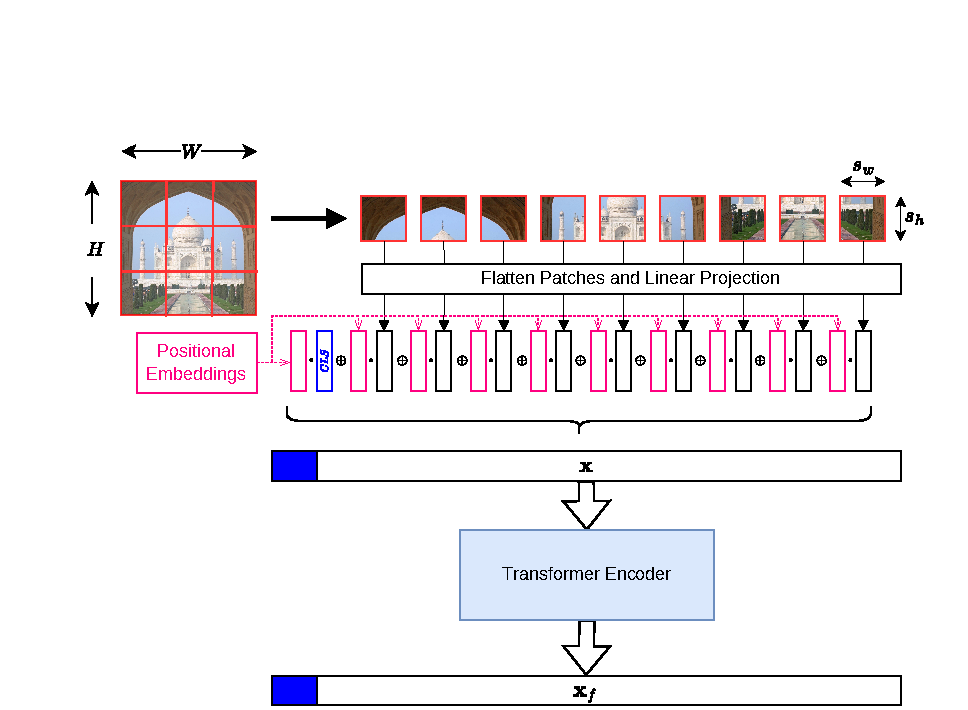
\includegraphics[width=\textwidth]{vision_transformer_img_overview.pdf}
    \caption{Data processing for Vision Transformers}
    \small
        Input image is first broken into patches. These patches are
        flattened and a (shared) linear projection is applied to all
        of them. A $\left[CLS\right]$ token is added for global
        context. Then, position embeddings are added to each element
        and the entire set in concatenated into a vector (with the
        $\left[CLS\right]$ - denoted in blue squared - usually going
        first). The $\cdot$ (dot) signifies addition of position
        embeddings and $\oplus$ signifies concatenation. \\
        Image is best viewed in color.
    \label{fig:vit_input_patchification}
\end{figure}

\paragraph{Step 1 - Patchification of the Input Image}

As shown in \cref{fig:vit_input_patchification}, an input image
$\mathbf{I} \in \mathbb{R}^{C, H, W}$ is split into patches of shape
$s_h, s_w$ each, giving $n_h = H/s_h$ patches along height and $n_w =
W/s_w$ patches along width. These $n = n_h \times n_w$ patches are
then flattened into $d_m = C \times s_h \times s_w$ dimensional
vectors. Each patch is multiplied by a \emph{shared} square linear
matrix, keeping the output dimensionality same. We obtain the
transformed patch embeddings as $\left\{ \mathbf{p}_i \in
\mathbb{R}^{d_m} \right\}_{i = [1, n]}$. For utilizing global context,
a learnable $\mathbf{p}_0 = \left[CLS\right]$ token (same shape as the
patch vectors) is added to the set. These $n+1$ patches are then
transformed by adding position embeddings (so that each element in the
sequence gets a notion of its position in the sequence). Finally,
they're all concatenated into a vector. The final input to the model
is given by the vector $\mathbf{x} \in \mathbb{R}^{(1+n) \times d_m}$
(with the first $d_m$ values for the $\left[CLS\right]$ token). This
vector $\mathbf{x}$ is the input to the transformer layers. For
simplicity, we use $l = 1 + n$ for sequence length hereon.

\begin{figure}
    \centering
    \includegraphics[width=\textwidth]{vision_transformer_encoder_mha.pdf}
    \caption{Transformer Encoder and Multi-Headed Attention}
    \small
        Each transformer encoder block contains multi-headed attention
        block. The $+$ operations denote addition of residuals. Each
        head has its own query $\mathbf{Q}_i$, key $\mathbf{K}_i$ and
        value $\mathbf{V}_i$ vectors and applies self-attention. \\
        Image is best viewed in color.
    \label{fig:vit_encoder_mha}
\end{figure}

\paragraph{Step 2 - Transformer Encoders with Multi-headed Attention}

As shown in figure \cref{fig:vit_encoder_mha}, the input is given to
$N$ transformer encoder blocks, which are linked in sequence. Each
block normalizes its input, passes it through a multi-headed attention
(MHA) layer in residual, it finally passes it through an MLP block in
the same normalization and residual manner. LayerNorm
\cite{Ba2016LayerN} is used instead of BatchNorm
\cite{Ioffe2015BatchNA} because it is easier to parallelize and can
deal with varying batch sizes. Each head (say head $i$) of MSA does
the following

\begin{enumerate}
    \item The input $\mathbf{x} \in \mathbb{R}^{l, d_m}$ (where $l =
        1+n$ is the sequence length and $d_m$ is the feature
        dimension) is passed through LayerNorm, giving
        $\tilde{\mathbf{x}} = \mathrm{LN}(\mathbf{x})$ (where
        $\tilde{\mathbf{x}} \in \mathbb{R}^{l, d_m}$). We then apply
        weights $\mathbf{W}_{Qi} \in \mathbb{R}^{d_m, d_k}$ for query,
        $\mathbf{W}_{Ki} \in \mathbb{R}^{d_m, d_k}$ for key, and
        $\mathbf{W}_{Vi} \in \mathbb{R}^{d_m, d_k}$ for value. Here,
        $d_k = d_m / h$, where $h$ is the number of heads ($h$ is
        chosen such that it divides $d_m$). We get the query
        $\mathbf{Q}_i \in \mathbb{R}^{l, d_k}$, key $\mathbf{K}_i \in
        \mathbb{R}^{l, d_k}$, and value $\mathbf{V}_i \in
        \mathbb{R}^{l, d_k}$ vectors using
        \begin{align}
            \mathbf{Q}_i &= \tilde{\mathbf{x}} \mathbf{W}_{Qi} &
            \mathbf{K}_i &= \tilde{\mathbf{x}} \mathbf{W}_{Ki} &
            \mathbf{V}_i &= \tilde{\mathbf{x}} \mathbf{W}_{Vi}
        \end{align}
    
    \item The output of the self-attention $\mathbf{A}_{i} \in
        \mathbb{R}^{l, d_k}$ is given
        by
        \begin{align}
            \mathbf{A}_i = \mathrm{Attention}(\mathbf{Q}_i, 
                \mathbf{K}_i, \mathbf{V}_i) = \mathrm{softmax} \left(
                    \frac{\mathbf{Q}_i \mathbf{K}_i^\textup{T}}
                        {\sqrt{d_k}}\right) \mathbf{V}_i
        \end{align}
        The above equation is similar to information retrieval where a
        query is matched with key using $d_k$ dimensional embeddings
        to retrieve value (information). This formulates it in a
        differentiable and continuous manner. The $\mathrm{softmax}$
        uses $\sqrt{d_k}$ for normalization and does row-wise
        normalization.
    
    \item The output across all heads is concatenated (along the $d_k$
        dimension of each vector) into a single vector $\mathbf{A} \in
        \mathbb{R}^{l, d_m}$ using
        \begin{equation}
            \mathbf{A} = \left[\mathbf{A}_1 \oplus \mathbf{A}_2 \oplus 
                \cdots \oplus \mathbf{A}_i \oplus \cdots \mathbf{A}_h
                \right]
        \end{equation}
    
    \item The final output $\mathbf{y} \in \mathbb{R}^{l, d_m}$ of the
        MHA block is given by applying a linear transformation through
        weights $\mathbf{W}_O \in \mathbb{R}^{d_m, d_m}$, given by
        \begin{equation}
            \mathbf{y} = \mathbf{A} \mathbf{W}_O
        \end{equation}
        The weights $\mathbf{W}_O$ mix the outputs across all heads.
\end{enumerate}

\paragraph{Step 3 - Normalize and Linear Transform}

The output of MHA block $\mathbf{y} \in \mathbb{R}^{l, d_m}$ is then
added with the input $\mathbf{x} \in \mathbb{R}^{l, d_m}$ (residual
connection). The result is then passed through LayerNorm
\cite{Ba2016LayerN} (along the $d_m$ dimension) and then a 2-layer MLP
where first layer expands the dimension from $d_m$ to $4d_m$, and the
second layer reduces the dimension form $4d_m$ to $d_m$. The result is
added with a residual connection, shown in \cref{fig:vit_encoder_mha}.
This gives the output $\mathbf{z} \in \mathbb{R}^{l, d_m}$ of the
current layer (which is then the input for the next layer).

\begin{equation}
    \mathbf{z}_{out} = \mathrm{MLP}(
        \mathrm{LN}(\mathbf{y} + \mathbf{x})) + 
        (\mathbf{y} + \mathbf{x}) \\
\end{equation}

\paragraph{Downstream Tasks}

The downstream tasks take the $\left[CLS\right]$ token (first $d_m$
values) and use it for classification (by adding an additional MLP)
\cite{Dosovitskiy2020AnII}. We explore the representations learned by
latent layers for visual place recognition.

\paragraph{Configurations} The ViT proposed by Google has variants
described in \cref{tab:vit_configs}. The input image size is $(224,
224)$. With patch size $(16, 16)$, it gives $d_m = 3 \times 16 \times
16 = 768$ dimensional patch embeddings. Architectures that have a
different embedding dimension (like ViT-L) use a non-square linear
projection at the input stage (as shown in
\cref{fig:vit_input_patchification}); these are usually used to
increase dimensionality. All entries are from \href{https://github.com/google-research/vision\_transformer/blob/3d8e81478e2f9f34e367ba661ee0cd02cd12ee6b/vit\_jax/configs/models.py}
{google-research/vision\_transformer on GitHub}.

\begin{table}
    \centering
    \begin{tabular}{cccccccc}
        \hline
        Family & Model & Params & Patch $s$ & Emb. $d_m$ & 
            Heads $h$ & Layers $N$ & MLP Block \\
        \hline
        \multirow{3}{*}{ViT \cite{Dosovitskiy2020AnII}} &
            ViT-B & 86M & 16 & 768 & 12 & 12 & (*-3072-*) \\
            & ViT-L & 307M & 16 & 1024 & 16 & 24 & (*-4096-*) \\
            & ViT-H & 632M & 14 & 1280 & 16 & 32 & (*-5120-*) \\
        \hline
        \multirow{3}{*}{DeIT \cite{Touvron2020TrainingDI}} &
            DeIT-Ti & 5M & 16 & 192 & 3 & 12 & (*-768-*) \\
            & DeIT-S & 22M & 16 & 384 & 6 & 12 & (*-1536-*) \\
            & DeIT-B & 86M & 16 & 768 & 12 & 12 & (*-3072-*) \\
        \hline
        \multirow{5}{*}{CCT \cite{Hassani2021EscapingTB}} &
            ViT-Lite-7/8 & 3.74M & 8 & 256 & 4 & 7 & (*-512-*) \\
            & ViT-Lite-7/4 & 3.72M & 4 & 256 & 4 & 7 & (*-512-*) \\
            & CVT-7/4 & 3.72M & 4 & 256 & 4 & 7 & (*-256-*) \\
            & CCT-2/3x2 & 0.28M & c(3x3)*2 & 128 & 2 & 2 & 
                (*-128-*) \\
            & CCT-7/3x1 & 3.76M & c(3x3) & 256 & 4 & 7 & (*-512-*) \\
        \hline
    \end{tabular}
    \caption{Transformer Variants and Specifications}
    \small
        Comparisons of different transformer configurations. Params
        signifies the number of parameters. The patch size is given by
        $s = s_h = s_w$ (square patches), $c(\cdot)$ means convolution
        tokenizer. MLP block specifications are given as
        $(input-hidden-output)$, a `*' here means `same as $d_m$'.
    \label{tab:vit_configs}
\end{table}

\subsection{DeIT}
\label{subsec:vit-deit}

Data efficient Image Transformers (DeIT) \cite{Touvron2020TrainingDI}
proposes minor modifications towards training transformers. Instead of
training on JFT-300M (like ViT), DeIT is trained only on ImageNet. It
uses the same architecture and improvements from the \texttt{timm}
(PyTorch Image Models) library \cite{Wightman2019PyTorchIM}. Compared
to ViT, DeIT also uses a lower batch size (1024 vs. 4096), learning
rate adjusted with batch size \cite{Goyal2017AccurateLM}, and
RandAugment data augmentation \cite{Cubuk2020RandaugmentPA}. Various
DeIT models are mentioned in \cref{tab:vit_configs} (taken from
\cite{Touvron2020TrainingDI} and
\href{https://github.com/facebookresearch/deit/blob/263a3fcafc2bf17885a4af62e6030552f346dc71/models.py}{facebookresearch/deit
GitHub}).

\paragraph{Distillation Models} DeIT also proposes a distillation
strategy for vision transformers where an extra distillation token is
added (like the class token), but is trained for a distillation loss
(like the KL divergence). Instead of using a \emph{soft distillation}
approach (modeling the softmax of teacher), they use a hard-label
distillation strategy where they use cross-entropy (CE) loss on the
teacher's label. More on knowledge distillation is mentioned in
\cref{subsec:fm-k-distill}.

\subsection{Other Model Architectures}

\paragraph{Swin Transformers \cite{Liu2021SwinTH}} Shifted Windows
(Swin) transformers constrains the self-attention to local windows.
This way, in a particular layer, only the patches within a local
window exchange information. This avoids the quadratic complexity of
applying global attention. Consecutive layers have shifted windows so
that information exchange happens through patches that enter or leave
windows. It also proposes merging patches to form hierarchical
representations.

\paragraph{Swin Transformer V2 \cite{Liu2021SwinTV}} improves the Swin
Transformer further by changing the pre-normalization to
post-normalization, replacing the dot-product to a scaled cosine
function in the attention formulation, and using log-space in
positional embeddings.

\paragraph{CCT \cite{Hassani2021EscapingTB}} aims to train vision
transformers on small datasets. It proposes ViT-Lite, Compact Vision
Transformers (CVT), and Compact Convolution Transformers (CCT). Its
variants are presented in \cref{tab:vit_configs}.

\emph{ViT-Lite} is a more suitable ViT architecture, nearly identical
to the original ViT, for small-scale learning. It achieves better
results using only 7 layers and a $4, 4$ patch size, while having 
fewer parameters.

\emph{CVT} removes the conventional $\left[CLS\right]$ token and
instead uses Sequence Pooling (SeqPool) to get the output. It uses a 
linear layer with $\mathrm{softmax}$ to generate weights for pooling
the output tokens.

\emph{CCT} uses a convolutional tokenizer in CVT. It replaces the
input embeddings (like in \cref{fig:vit_input_patchification}) with a
$\mathrm{conv}$ layer followed by $\mathrm{MaxPool}$. This adds
inductive biases of a convolution network in the transformer model.

\section{SSL Concepts}

\subsection{Knowledge Distillation}
\label{subsec:fm-k-distill}

In the field of deep learning, knowledge distillation refers to the
technique of transferring knowledge acquired by a pre-trained model
(teacher) to a new model (student) \cite{Hinton2015DistillingTK}. This
process aims to empower the student model to achieve performance
comparable to the teacher, often with a smaller and more efficient
architecture. During knowledge distillation, the student learns to
mimic the teacher's behavior, effectively leveraging the teacher's
knowledge to improve its own performance. Usually, a dataset split,
called the ``transfer set'', is used for this purpose. It is also
common to train the student model on the dataset after distillation or
concurrently. Most commonly, it is of three types

\begin{enumerate}
    \item Teacher-Student with different architectures: This scenario
        is commonly used when the teacher network is a large network
        trained on a significant amount of data, while the student
        network is a simpler model designed for deployment
        constraints. The student network is trained to mimic the
        softmax outputs (often just before the output layer) of the
        teacher on the transfer set.
    \item Teacher-Student with same architecture: This strategy aims
        for the student to learn robust representations from the
        training dataset.  Here, the teacher, often initialized with
        the same architecture as the student, is trained using an
        exponentially moving average (EMA) of the student gradients.
        Such techniques enable a fast-learning student to benefit from
        a teacher that has access to a more robust representation of
        the training data (through the EMA).
    \item Mixture-of-Experts teacher: This approach is typically used
        for very large datasets with many categories. A global
        generalist model is trained to identify categories within the
        data, and an expert model is trained on each category. The
        generalist model serves two key purposes: identifying
        sub-classes (gating mechanism) for a given sample and acting
        as a catch-all class for samples where no expert has a strong
        specialization. Samples from a transfer set are used to train
        a student model that must model the probability distribution
        of both the generalist and the relevant expert(s) for the
        category of the sample.
\end{enumerate}

\subsubsection{Loss for Learning Targets}

In knowledge distillation, the loss function plays a crucial role in
guiding the student model to mimic the knowledge of the teacher model.
There are two primary approaches for defining the target distribution
that the student should learn: soft targets and hard targets. Soft
target modeling is when the concerned probability distribution is a
softmax distribution over all output classes of the teacher. On the
other hand, hard target is when only the single output class (per
sample of the transfer set) is considered. Usually, losses like cross
entropy and Kullback-Leibler (KL) Divergence are used for this
alignment. These are derived from information theory, but fund use in
aligning probability distributions (like softmax outputs of a student
to align with the output of teacher).

\paragraph{Entropy} is a measure of useful information for a
probability of an event. For example, let $x$ be a random variable
modeling distribution $P(X)$, that is $x \sim P(X)$. The entropy
(information) of $x = E$, basically $P(X = E) = P(E)$ is given by

\begin{equation}
    I_{x \sim P}(E) = \mathrm{log}\left(\frac{1}{P(E)}\right)
        = -\mathrm{log}\left(P(E)\right)
\end{equation}

The expected entropy over all states/events of $x$ is the entropy of
the distribution $P$. It is given by

\begin{equation}
    \textup{H}_{x \sim P}(X) = \textup{E}_{x \sim P}\left(I(X)\right) 
        = \sum_{x \in X} P(X = x) I(X = x)
        = -\sum_{x \in X} p(x) \textup{log}(p(x))
\end{equation}

where $p(x) = P(X = x) \in \mathbb{R}$ is used to denote the
probability of the event $X = x$.

\paragraph{Kullback-Leibler Divergence} or KL Divergence is the excess
information required to model $X$ using distribution $Q(X)$, when the
actual (underlying) distribution is $P(X)$. It is used to measure the
deviation when using $x \sim Q$, if the actual distribution is
supposed to be $x \sim P$; it is a directed difference between two
distributions. It is modeled as

\begin{align}
    \textup{D}_{KL}(P \parallel Q) &= \textup{E}_{x \sim P} \left(
            I_{x\sim Q}(X = x) - I_{x\sim P}(X = x)\right)
        = \sum_{x \in X} P(X = x) \mathrm{log}\left(
            \frac{P(X = x)}{Q(X = x)}\right) \nonumber \\
        &= \sum_{x \in X} p(x) \mathrm{log}\left(\frac{p(x)}{q(x)}
            \right)
        = -\sum_{x \in X} p(x) \mathrm{log}\left(\frac{q(x)}{p(x)}
            \right)
\end{align}

where $q(x) = Q(X = x) \in \mathbb{R}$ is used to denote the
probability of the event $X = x$ (using distribution $Q(X)$). The
above is easy to differentiate with respect to $q(x)$ and it is
ideal to have $q(x)$ for the student and $p(x)$ for the teacher.

\paragraph{Cross Entropy} is defined as the difference between two
distributions for a specific event. It is the excess information
needed for encoding $Q$, when the underlying distribution is $P$.
It is formulated as

\begin{align}
    \textup{H}(p, q) &= \textup{H}(p) + \textup{D}_{KL}(p \parallel q)
        = \sum_{x \in X} p(x) \mathrm{log}\left(\frac{1}{p(x)}\right)
            + \sum_{x \in X} p(x) \mathrm{log}\left(\frac{p(x)}{q(x)}
                \right) \nonumber \\
        &= \sum_{x \in X} p(x) \mathrm{log}\left(\frac{1}{q(x)}\right)
        = -\sum_{x \in X} p(x) \mathrm{log}\left(q(x)\right)
\end{align}

This is more directly related to the entropy of $Q$ and the likelihood
of $P(X=x)$ and is more commonly used to align a student (as $q(x)$)
to a teacher (as $p(x)$).

\section{DINO and DINOv2 Models}

\subsection{DINO}
\label{subsec:fm-dino}

DINO \cite{Caron2021EmergingPI}, distillation with no labels, is a
method of knowledge distillation where the student and the teacher
have the same architecture and where the \emph{cross entropy loss} is
used for aligning the student to the teacher and where the teacher is
the EMA of the student network. Using the multi-crop strategy
\cite{Caron2020UnsupervisedLO}, a set of views $V$ is generated from
an image. Two of these views are large global crops ${x_1^g, x_2^g}$
and others are smaller resolution local views. The student network is
given by $P_s$ and the teacher is given by $P_t$ (both have the same
architecture). The training loss is minimized as follows

\begin{equation}
    \underset{\theta_s}{\textup{min}} \sum_{x \in \{x_1^g, x_2^g\}}
        \sum_{\overset{x' \in V}{x' \neq x}} H(P_t(x), P_s(x'))
\end{equation}

Note that the teacher gets no gradient. In PyTorch, it's implemented
using a \texttt{detach} call to the output. The teacher is updated
using an exponentially moving average (momentum encoder)
\cite{He2019MomentumCF} of the student weights, given by $\theta_t
\leftarrow \lambda \theta_t + (1 - \lambda) \theta_s$. 
To avoid collapse of outputs (preventing one dimension to dominate
over the others or the output becoming a uniform distribution), the
teacher's output is centered (with the center in-turn being updated as
an EMA of teacher's outputs) and sharpened using temperature softmax.

The architecture is DeIT from \cref{subsec:vit-deit}, with patch size
8 and the transformer having a pre-norm layer normalization. The main
work of DINO uses a $\left[CLS\right]$ token and applies a linear
projection head or employs k-NN (k nearest neighbor) for
classification. However, we are more interested in features learned
by the latent (intermediate) transformer layers. Especially for the
context of VPR.

DINO demonstrates that self-supervised learning using the ViT
architecture could form a strong vision foundation model that can be
used for downstream tasks.

\subsection{Further Developments}

\subsubsection{iBOT}
\label{subsec:fm-ibot}

Image BERT pre-training with Online Tokenizer (iBOT)
\cite{Zhou2021iBOTIB} takes inspiration from Masked Language Modeling
(MLM) in BERT \cite{Devlin2019BERTPO} to perform Masked Image Modeling
(MIM). It formulates MIM task as a knowledge distillation (KD) task
with an online tokenizer (used to transform the patches) trained
simultaneously with the target model. The MIM task is also solved in
BEiT (BERT Pre-Training of Image Transformers) \cite{Bao2021BEiTBP},
albeit with an offline tokenizer learned from visual vocabulary.

During training, block-wise masking is performed on the input image
and two augmented views $\mathbf{u}$ and $\mathbf{v}$ are generated
with their corresponding masked views $\hat{\mathbf{u}}$ and
$\hat{\mathbf{v}}$. The student and the teacher have a transformer
backbone and a shared projection head (which is an MLP) for patch
tokens and $\left[CLS\right]$. The losses contain distillation across
the same view and cross-view, for the MIM objective and the
$\left[CLS\right]$ objective. For the MIM task, the objective is to
align the predicted softmax of the masked tokens (where $m_i = 1$).
The cross-entropy (CE) objectives are given as

\begin{align}
    \mathrm{L}_{MIM}^{u_t \rightarrow \hat{u}_s} &= -\sum_{i = 1}^{N}
        m_i \textup{P}_{\theta'}^t\left(\mathbf{u}_t^{patch}\right)^{
            \top} \mathrm{log} \left( \textup{P}_{\theta}^s 
            \left(\hat{\mathbf{u}}_s^{patch}\right)\right) &
    \mathrm{L}_{\left[CLS\right]}^{u_t \rightarrow \hat{v}_s} &=
        - \textup{P}_{\theta'}^{t} \left(
            \mathbf{u}_t^{\left[CLS\right]}\right) \mathrm{log} \left(
            \textup{P}_{\theta}^s\left(\hat{\mathbf{v}}_s^{
            \left[CLS\right]}\right)\right) \nonumber \\
    \mathrm{L}_{MIM}^{v_t \rightarrow \hat{v}_s} &= -\sum_{i = 1}^{N}
        m_i \textup{P}_{\theta'}^t\left(\mathbf{v}_t^{patch}\right)^{
            \top} \mathrm{log} \left( \textup{P}_{\theta}^s 
            \left(\hat{\mathbf{v}}_s^{patch}\right)\right) &
    \mathrm{L}_{\left[CLS\right]}^{v_t \rightarrow \hat{u}_s} &=
        - \textup{P}_{\theta'}^{t} \left(
            \mathbf{v}_t^{\left[CLS\right]}\right) \mathrm{log} \left(
            \textup{P}_{\theta}^s\left(\hat{\mathbf{u}}_s^{
            \left[CLS\right]}\right)\right)
\end{align}

Where $\mathrm{L}^{a \rightarrow b}$ denotes distillation from teacher
$a$ to student $b$, and $\mathrm{L}_{MIM}$ and $\mathrm{L}_{
\left[CLS\right]}$ are MIM tokens and CLS token losses respectively.
As in DINO, the teacher is an EMA of student, updated through momentum
of student weights. iBOT is able to form robust representations
suitable for many downstream tasks such as object detection, panoptic
segmentation, and transfer learning. The patch tokens learn
semantically meaningful information that contains global context
(because of the shared head with $\left[CLS\right]$ and the online
tokenizer).

\subsubsection{DINOv2}
\label{subsec:fm-dinov2}


DINOv2 \cite{Oquab2023DINOv2LR} contains an automatic pipeline to
build a rich and diverse training dataset, and a distillation stage
from a large model. It performs significantly better than CLIP
\cite{Radford2021LearningTV} on benchmarks needing local and global
semantic information.

Following \cite{Pizzi2022ASD}, a curated dataset is first built by
starting with little curated data. Embeddings are extracted from
curated and un-curated data. Duplicates in the un-curated data (having
close embeddings) are removed. Those samples that can be retrieved
from the remaining un-curated set by querying embeddings from the
curated set are added to the augmented curated set. The dataset source
includes ImageNet, Google Landmarks, and many fine-grained datasets
like ADE-20K, Pascal VOC, CityScapes, etc. The final dataset is called
LVD-142M.

DINOv2 uses the same image-level objective from DINO (in
\cref{subsec:fm-dino}) and patch-level objective from iBOT (in
\cref{subsec:fm-ibot}): cross entropy losses, knowledge distillation
setting, teaching being the EMA of student. Other than this, DINOv2
has several improvements

\begin{enumerate}
    \item Unlike the shared projection heads in iBOT, it \emph{unties}
        (separates) the heads for patch and image-level objective.
    \item Instead of applying softmax and centering to the teacher's
        output, \emph{Sinkhorn-Knopp centering} is applied for 3
        iterations. During training, the activations for each
        mini-batch are L2-normalized and a pair-wise similarity matrix
        is computed. This similarity matrix is steered to a template.
        The student goes through only softmax-norm. This is inspired
        from SwAV \cite{Caron2020UnsupervisedLO}.
    \item Uses \emph{KoLeo Regularizer}
        \cite{Sablayrolles2018SpreadingVF}: Given a set of vectors
        (activations for a minibatch) $\{x_1, x_2, \cdots, x_n\}$, it
        defines a loss $L_{koleo} = -\frac{1} {n} \sum_{i=1}^n
        \mathrm{log}(d_{n, i})$ where $d_{n, i} = \textup{min}_{j \neq
        i} \left\|x_i - x_j\right\|$ is the minimum distance between
        samples in the minibatch. This aims to spread out samples in
        each batch.
    \item Using Swish Gated Linear Unit (SwiGLU) activations
        \cite{Shazeer2020GLUVI} for the FFN in the transformer layers.
    \item Using \emph{Stochastic Depth} \cite{Huang2016DeepNW} to
        shrink the depth of a network during training (by randomly
        dropping entire residual blocks and replacing it with a
        bypass) while keeping it the same during inference. It helps
        the network learn sophisticated representations in earlier
        layers.
    \item Using \emph{LayerScale} \cite{Touvron2021GoingDW} to train
        deep transformer models (with many layers). It adds a
        learnable diagonal matrix (multiplication) to the output of
        the residual blocks. This has been shown to increase model
        capacity.
    \item Training a large ViT-g network (with 1.1B parameters) from
        scratch and then training smaller models through knowledge
        distillation \cite{Hinton2015DistillingTK}. It trains a
        ViT-g/14 from scratch on LVD-142M and uses this as the frozen
        teacher for the initial stages of training smaller ViT models
        (like ViT-L/14, ViT-B/14, and ViT-S/14).
    \item Using higher-resolution images (518, 518) during the end of
        pre-training. Additionally, using a patch size of 14 seems to
        give better results.
\end{enumerate}

Additionally, efficient implementation with \texttt{xFormers}
\cite{Lefaudeux2022xFormersAM}, \texttt{timm}
\cite{Wightman2019PyTorchIM}, and \texttt{FairScale}
\cite{FairScale2021} libraries bring the following changes

\begin{enumerate}
    \item Improved computational efficiency and resource utilization
        using FlashAttention \cite{Dao2022FlashAttentionFA}: it breaks
        the attention matrix operation into smaller chunks (called
        tiles) and optimizes the memory R/W operations on the GPU
        (between HBM and SRAM).
    \item Nested Tensors allow modeling tensors with varying sequence
        length more efficiently (by containerizing each element as a
        Tensor).
    \item Using PyTorch FSDP (Fully Sharded Data Parallel)
        \cite{Zhao2023PyTorchFE} to split the model and data across
        GPUs and to reduce cross-GPU communication. This relates to
        data sharding (splitting across databases) in large database
        management systems, but it splits the model's parameters into
        shards (splits), usually along feature dimensions.
\end{enumerate}

The above improvements lead to better representations learned by
DINOv2 and make its training more efficient. It performs much better
than DINO \cite{Caron2021EmergingPI}, MAE \cite{He2021MaskedAA}, and
iBOT \cite{Zhou2021iBOTIB} on ImageNet, and has better linear
evaluation over frozen features (linear probing) on fine-grained
benchmarks. It also performs better on tasks like semantic
segmentation, depth estimation, and image retrieval.

We are interested in exploiting latent features learned by
intermediate transformer layers of DINOv2 for the purpose of visual
place recognition (VPR). We show that these learn more meaningful
representations and can be clubbed with existing feature aggregation
techniques.


% --------------------- Chapter ---------------------
\chapter{AnyLoc: Foundation Model features for VPR}
\label{ch:anyloc}
% !TEX root = ./main.tex

% ---------------- Macros ----------------
% Colors
\definecolor{OutdoorDark}{rgb}{0,.5,0}
\definecolor{IndoorDark}{rgb}{0,0.3,0.8}
\definecolor{SubTDark}{rgb}{0.5,.27,0.11}
\definecolor{AerialDark}{rgb}{.5,.0,.5}
\definecolor{UnderWaterDark}{rgb}{0.16, 0.46, 0.81}
\colorlet{Outdoor}{OutdoorDark!20!white}
\colorlet{Indoor}{IndoorDark!20!white}
\colorlet{SubT}{SubTDark!20!white}
\colorlet{Aerial}{AerialDark!20!white}
\colorlet{UnderWater}{UnderWaterDark!20!white}
\colorlet{OutdoorLight}{OutdoorDark!70!white}
\colorlet{IndoorLight}{IndoorDark!70!white}
\colorlet{SubTLight}{SubTDark!70!white}
\colorlet{AerialLight}{AerialDark!70!white}
\colorlet{UnderWaterLight}{UnderWaterDark!70!white}
% Symbols
\newcommand{\symbolHt}{1.2em}
\newcommand{\oppsymbolHt}{1em}
\newcommand{\outdoorChar}{%
    \begingroup\normalfont
    \includegraphics[height=\symbolHt]{symbols/outdoor.png}%
    \endgroup
}
\newcommand{\indoorChar}{%
    \begingroup\normalfont
    \includegraphics[height=\symbolHt]{symbols/indoor.png}%
    \endgroup
}
\newcommand{\subtChar}{%
    \begingroup\normalfont
    \includegraphics[height=\symbolHt]{symbols/cave.png}%
    \endgroup
}
\newcommand{\hawkinsChar}{%
    \begingroup\normalfont
    \includegraphics[height=\symbolHt]{symbols/degraded.png}%
    \endgroup
}
\newcommand{\aerialChar}{%
    \begingroup\normalfont
    \includegraphics[height=\symbolHt]{symbols/aerial.png}%
    \endgroup
}
\newcommand{\underwaterChar}{%
    \begingroup\normalfont
    \includegraphics[height=\symbolHt]{symbols/underwater.png}%
    \endgroup
}
\newcommand{\viewpointChar}{%
    \begingroup\normalfont
    \includegraphics[height=\symbolHt]{symbols/viewpoint.png}%
    \endgroup
}
\newcommand{\lightingChar}{%
    \begingroup\normalfont
    \includegraphics[height=\symbolHt]{symbols/day_night.png}%
    \endgroup
}
\newcommand{\oppositeChar}{%
    \begingroup\normalfont
    \includegraphics[height=\oppsymbolHt]{symbols/opp_viewpoint.png}%
    \endgroup
}
% ----------------------------------------


Prior Visual Place Recognition (VPR) methods have shown great
performance when tackling task-specific challenges in isolation. A
generic out-of-the-box model will need to perform adequately well
under a large set of challenges, including cases where there isn't
enough data for training or when training on different domains is
complex. This chapter introduces AnyLoc \cite{Keetha2023AnyLocTU}
which is the first step towards a universal VPR system.

VPR task is defined in \cref{subsec:intro-vpr}. AnyLoc aims to solve
image retrieval over a wide range of dataset settings using an
off-the-shelf foundation model without any VPR-specific fine-tuning.

\section{Prior Knowledge}

\subsection{VPR Baselines}

Global image descriptors are already described in
\cref{subsec:intro-vpr}. We choose to compare with the following
prominent baselines that are widely used in the VPR community.

\paragraph{NetVLAD \cite{Arandjelovi2015NetVLADCA}} is a smooth
(differentiable) version of VLAD (Vector of Locally Aggregated
Descriptor). It is a weakly supervised contrastive learning method
where the positive and negatives are mined by proximity (geographical
distance). It is trained on the Pitts-250k dataset
\cite{Torii2013VisualPR}. A major drawback is the negative mining
technique that is infeasible in large scale settings and the high
dimensional embeddings that lose significant performance when
dimensionality reduction techniques like PCA are applied.

\paragraph{CosPlace \cite{Berton2022RethinkingVG}} proposes a
city-wide visual geo-localization solution by casting the training
process as a classification problem. Itt partitions the dataset into
classes based on the location (geographical coordinates) and the
heading, and groups neighboring classes into groups. It then applies
the Large Margin Cosine Loss (LCML), also known as CosFace
\cite{Wang2018CosFaceLM}, sequentially over each group; this loss
introduces a cosine margin (through dot product) in the normalized
version of the Softmax loss. CosPlace uses GeM pooling with output
dimension 512 (much lesser than NetVLAD). It also proposes the San
Francisco extra large (SF-XL) dataset for benchmarking city-wide VPR.

\paragraph{MixVPR \cite{Alibey2023MixVPRFM}} proposes a feature
aggregation technique without self-attention or regional pooling,
inspired by MLP-Mixer \cite{Tolstikhin2021MLPMixerAA}. MLP-Mixer
contains channel-mixing and token-mixing MLP layers. Given a tokenized
input (like in the first step of the transformer) $\mathbf{X} \in
\mathbb{R}^{S, C}$, the mixer does channel-mixing to get
$\mathbf{U} \in \mathbb{R}^{S, C}$ and token-mixing to get
$\mathbf{V} \in \mathbb{R}^{S, C}$, given by

\begin{align}
    \mathbf{U}[:, i] &= \mathbf{X}[:, i] + \mathbf{W}_2 \sigma \left(
        \mathbf{W}_1 \mathrm{LN}\left(\mathbf{X}[:, i]\right)\right),
        \qquad \textup{for}\: i = 1 \dots C \\
    \mathbf{Y}[j, :] &= \mathbf{U}[j, :] + \mathbf{W}_4 \sigma \left(
        \mathbf{W}_3 \mathrm{LN}\left(\mathbf{U}[j, :]\right)\right),
        \qquad \textup{for}\: j = 1 \dots S
\end{align}

This gives the network linear complexity in terms of number of patches
(unlike the quadratic complexity of the attention mechanism) and the
number of pixels in the input image. MixVPR first extract feature maps
from intermediate layers of a CNN backbone, it then feeds these to a
feature mixing block (consecutive MLP blocks) to incorporate global
relationship in each feature map. MLPs are used to reduce the
dimensionality (both row-wise and column-wise) and the final output is
flattened and L2-normalized, giving the global descriptor for the
input image. It is trained using Multi-Similarity Loss
\cite{Wang2019MultiSimilarityLW} using the GSV-Cities framework
\cite{Alibey2022GSVCitiesTA}.

\subsection{Foundation Models}

This is discussed in detail in \cref{ch:foundation-models}. We
benchmark the capability of the following vision foundation models.

\paragraph{CLIP \cite{Radford2021LearningTV}} is an image captioning
model that is trained to align embeddings from a text and an image
backbone. A dataset is distilled from YFCC100M
\cite{Thomee2015YFCC100M} (filter images with English titles and
descriptions) to get around 15M images (about the size of ImageNet).
The text encoder is a modified transformer with some modifications
\cite{Radford2019LanguageMA, Vaswani2017AttentionIA}. The vision
encoder is either a ResNet \cite{He2015DeepRL} or ViT
\cite{Dosovitskiy2020AnII}. A minibatch contains a set of $(image,
text)$ pairs, the distance between the corresponding pairs should be
minimized while the non-corresponding pairs should be maximized. This
type of contrastive setting is carried out over a very large batch
size (of over 32,000). We ultimately get a trained visual encoder that
can understand the contents of an image by language supervision.

\paragraph{DINO \cite{Caron2021EmergingPI} and DINOv2
\cite{Oquab2023DINOv2LR}} are described in \cref{subsec:fm-dino} and
\cref{subsec:fm-dinov2} respectively. They use knowledge distillation
formulation (student-teacher with the same ViT architecture) with the
cross entropy loss to learn representations of an image. DINO uses a
simple DeIT implementation of ViT and ImageNet dataset, while DINOv2
uses a custom ViT implementation with many changes (to accommodate for
the much larger model size) and a curated dataset LVD-142M.

Prior work \cite{Amir2021DeepVF} shows that DINO features (from the
intermediate layers of the transformer) can be used to solve a range
of tasks that require semantic understanding of the image, for
example: co-segmentation of foreground, part co-segmentation, and
image part correspondences.

\section{AnyLoc: Towards Universal VPR}

\begin{figure}
    \centering
    \includegraphics[trim={0cm 9.7cm 0cm 0cm},clip,
        width=0.96\linewidth]{splash.pdf}
    \caption{AnyLoc: Anywhere, Anytime, and Anyview VPR}
    \small
        \emph{Left}: Image samples from various datasets used (and the
        legend for symbols and colors). \emph{Center}: Comparing the
        PCA projections of MixVPR (a supervised baseline) and AnyLoc
        (foundation model features). \emph{Right}: VPR performance by
        the test setting. Image from \cite{Keetha2023AnyLocTU} 
        (original paper).
    \label{fig:anyloc}
\end{figure}

AnyLoc aims to perform good image retrieval (VPR) in diverse places
(anywhere), under environmental changes (anytime), and under high
viewpoint changes (anyview). For this, we extract the representations
learned by the intermediate, often penultimate, transformer layers of
DINO and DINOv2. We find that conventional feature aggregation
techniques like VLAD and GeM, described in \cref{subsec:intro-vpr},
bring significant benefit over using only the output
$\left[CLS\right]$ token of these models. Our method, when projected
to 2D, also discovers unique features that distinguish and group
datasets of similar domain, which is lacking in most recent VPR
methods (see center of \cref{fig:anyloc} for comparison with MixVPR).
The process and steps for AnyLoc are described below

\subsection{Constructing AnyLoc Pipeline}

\subsubsection{Choice of Foundation Model}

From CLIP \cite{Radford2021LearningTV}, MAE \cite{He2021MaskedAA},
DINO \cite{Caron2021EmergingPI}, and DINOv2 \cite{Oquab2023DINOv2LR},
AnyLoc employs DINO and DINOv2 ViTs for extracting features. This is
because DINO and DINOv2 are trained for representation learning
(through knowledge distillation - as described in
\cref{subsec:fm-dino} and \cref{subsec:fm-dinov2}). CLIP is trained
on alignment and is used as a benchmarking method. MAE is trained to
in-fill masked tokens (like the MIM objective in iBOT and DINOv2) and 
without any special dataset curation. We find CLIP and DINO methods
perform better than pure masked modeling of MAE.

We use \emph{DINO} and \emph{DINOv2} models for extracting
intermediate features and CLIP for benchmarking.

\subsubsection{Choosing Layer and Facet}

A vision transformer, described in \cref{subsec:vit}, patchifies an
input image and passes it through layers of transformer encoder. The
transformer encoder consists of multi-headed self-attention (MHA)
modules (alongside the normalization, residual, and FFN blocks). Each
MHA has a softmax self-attention mechanism. The input to attention
are the \texttt{query}, \texttt{key}, and \texttt{value} facets. The
output of each transformer encoder (layer) is called the 
\texttt{value} facet.

\paragraph{Description}

Let the input to the model be $\mathbf{x}^{(0)} \in \mathbb{R}^{n,
d_m}$ and the input to the $l$-th transformer encoder layer be
$\mathbf{x}^{(l-1)} \in \mathbb{R}^{n, d_m}$ (also the output of the
previous layer). This goes through a normalization layer as
\begin{math}
    \bar{\mathbf{x}}^{(l-1)} = \textup{LN}(\mathbf{x}^{(l-1)}) \in
        \mathbb{R}^{n, d_m}
\end{math}
and projected to the query, key, and value facets as follows

\begin{align}
    \mathbf{q}^l &= \bar{\mathbf{x}}^{(l-1)} \mathbf{W}_{ql} &
    \mathbf{k}^l &= \bar{\mathbf{x}}^{(l-1)} \mathbf{W}_{kl} &
    \mathbf{v}^l &= \bar{\mathbf{x}}^{(l-1)} \mathbf{W}_{vl}
\end{align}

Where $\mathbf{W}_{ql}, \mathbf{W}_{kl}, \mathbf{W}_{vl} \in
\mathbb{R}^{d_m, d_m}$ are the projection weights. These facets are
split into $h$ heads and attention is applied to each head. The output
of the attention's softmax is added with $\mathbf{x}^{(l-1)}$. This
goes through another layer normalization and FFN (in a residual) and
the final output of layer $l$ is given as $\mathbf{x}^{(l)}$.

We say $\mathbf{q}^l$ is query, $\mathbf{k}^l$ is key, $\mathbf{v}^l$
is value, and $\mathbf{x}^l$ is token facet of the $l$-th layer. Each
is of type $\mathbb{R}^{n, d_m}$ ($n$ tokens, $d_m$ dimension each)
and is a candidate for feature aggregation.

\begin{figure}
    \centering
    \begin{subfigure}[b]{0.49\textwidth}
        \centering
        \includegraphics[trim={0cm 3.4cm 0cm 2.7cm},clip,
            width=0.95\linewidth]{facet_sim.pdf}
        \caption{Facet}
    \end{subfigure}
    \hfill
    \begin{subfigure}[b]{0.49\textwidth}
        \centering
        \includegraphics[trim={0cm 2.05cm 0cm 1.9cm},clip,
            width=0.95\linewidth]{facet_sim_layer_ablation.pdf}
        \caption{Layer}
    \end{subfigure}
    \caption{Facet and Layer-wise Attention Maps for DINOv2}
    \small
        \emph{Left}: Given a query point in the database image,
        various facets show different levels of contrast (with the
        most similar marker on the query image). Top has high scale
        change, middle has rotation change, and bottom has high
        perspective change. 
        \emph{Right}: A similar comparison across layers shows varying
        contrast. Notice that layer 31 shows the building (for the
        queried point in database image) with the best contrast.
    \label{fig:anyloc_facet_layer}
\end{figure}

\paragraph{Process} Given a dataset containing database and query
images, we pick a representative sample and pick a few corresponding
points. As seen in \cref{fig:anyloc_facet_layer}, a point in the left
database image is chosen and all patches (across all facets) are
extracted from the query image (on the right) and matched. A map
highlighting the similarity of each patch to the queried point is
visualized across facets and layers. The most similar patch is 
highlighted in the query image. On inspecting the similarity maps, we
can arrive at a decision on using a particular facet and layer. In the
case of \cref{fig:anyloc_facet_layer}, we choose the \texttt{value}
facet of the 31st layer (because the maps are most contrastive).


\subsubsection{Choosing Aggregation Method}

The facet features correspond to the individual patches of the image
(mostly local features with some semantic image information imbibed
due to training). These local features have to be aggregated to obtain
image-level features (also called global descriptors). These
techniques are described in \cref{subsec:intro-vpr}. We explore the 
following methods

\paragraph{VLAD} Vector of Locally Aggregated Descriptor is formed by
computing a vocabulary from a database of images, like the cluster
centers by clustering the local features. Given an image, the features
are assigned to the clusters and a residual is calculated (distance to
the cluster centers). The residuals are then aggregated for each
cluster, normalized, concatenated into one vector, and normalized
again.

Given features $\mathbf{f} \in \mathbb{R}^{n, d_m}$ (which could come 
from any facet of any layer mentioned earlier), we first get the
residual matrix $\mathbf{V} \in \mathbb{R}^{K, d_m}$

\begin{equation}
    \mathbf{V}[k, :] = \sum_{i=1}^{n} m_{i,k} (\mathbf{f}[i, :] - 
        \mathbf{c}[k, :])
\end{equation}

where $\mathbf{c} \in \mathbb{R}^{K, d_m}$ is the vocabulary of $K$
cluster centers, each $d_m$ dimensional. And $m_{i, k} = 1$ if feature
$i$ is assigned to cluster $k$ (closest to the cluster) and 0
otherwise.

\paragraph{Soft VLAD} replaces the $m_{i, k}$ with a softmax on the
distance between the feature $i$ and every cluster center $k$. This
gives distance-proportional assignment of every descriptor to every
cluster center. This is similar to the formulation of NetVLAD.

\paragraph{GeM} applies a mean pooling over the descriptors
$\mathbf{f} \in \mathbb{R}^{n, d_m}$ and gives pooled descriptor
$\mathbf{f}_G \in \mathbb{R}^{n, d_m}$ using

\begin{equation}
    \mathbf{f}_G = \left(\frac{1}{n} \sum_{i=1}^{n} \left(
            \mathbf{f}[i,:]\right)^p \right)^{\frac{1}{p}}
\end{equation}

\subsubsection{Choosing Vocabulary}

Algorithms like VLAD require a set of database images to form cluster
centers (vocabulary). We aim to characterize distinctive semantic
properties in a diverse set of environments. From \cref{fig:anyloc},
it is apparent that projecting the global descriptors of different
datasets highlights distinct domains in the latent space, allowing
us to characterize and group datasets having similar properties. 

The vocabulary is a superset (a collection of datasets) of images we
use to build database descriptors (for aggregation technique VLAD). We 
define the following types of vocabulary

\begin{itemize}
    \item \emph{Global}: Where database images from all the datasets
        are included when clustering.
    \item \emph{Structured}: Where only the database images from
        structured environments are included for clustering. These are
        outdoor and indoor datasets. These are most widely benchmarked
        in the VPR community and are from mostly human maintained
        environments.
    \item \emph{Unstructured}: Where database images from unstructured
        environments are included. These are subterranean, degraded,
        aerial, and underwater datasets. These aren't frequently
        benchmarked and remain less explored, but are important in
        scenarios like remote monitoring.
    \item \emph{Map-Specific} or dataset-specific: Where the database
        images from only the single dataset (which is being tested on)
        is used. For example, if the testing is on Oxford cars (an
        outdoor dataset), then the database images only from Oxford
        car are used to get the cluster centers for VLAD.
    \item \emph{Domain-Specific}: A domain is a collection of datasets
        with similar properties. The latent representation of AnyLoc
        descriptors allows us to discover these groups by clustering
        image descriptors from various datasets (as shown in
        \cref{fig:anyloc}). For example, for the outdoor domain, we
        use all the datasets captured in the outdoor setting.
\end{itemize}

\section{Experimental Setup}

\subsection{Datasets}

\begin{table}
    \centering
    \begin{tabular}{|ccccc||ccccc|}
        \hline
        \multicolumn{5}{|c|}{\textbf{Structured}} &
        \multicolumn{5}{|c|}{\textbf{Unstructured}} \\
        \hline
        \textbf{Dataset} & $\mathbf{N_{Db}}$ & $\mathbf{N_q}$ & 
            \textbf{Loc.} & \textbf{Type} &
        \textbf{Dataset} & $\mathbf{N_{Db}}$ & $\mathbf{N_q}$ & 
            \textbf{Loc.} & \textbf{Type} \\
        \hline
        {\color{IndoorDark} Baidu} \cite{Sun2017ADF} & 689 & 2292 & 
            10 m & \indoorChar &
        {\color{SubTDark} Hawkins} \cite{Zhao2023SubTMRSDP} & 65 & 
            101 & 8 m & \hawkinsChar \\
        {\color{IndoorDark} Gardens} \cite{Glover2021DayAN, 
            Snderhauf2015OnTP} & 200 & 200 & 5 fr & \indoorChar &
        {\color{SubTDark} Laurel} \cite{Zhao2023SubTMRSDP} & 141 & 
            112 & 8 m & \subtChar \\
        {\color{IndoorDark} 17 Places} \cite{Sahdev2016IndoorPR} & 
            406 & 406 & 5 fr & \indoorChar &
        {\color{AerialDark} Nardo-Air} \cite{He2023FoundLocVO} & 
            102 & 71 & 60 m & \aerialChar \\
        {\color{OutdoorDark} Pitts-30k} \cite{Torii2013VisualPR} & 
            10k & 6816 & 25 m & \outdoorChar &
        {\color{AerialDark} VP-Air} \cite{Schleiss2022VPAIRA} & 
            2.7k & 2.7k & 3 fr & \aerialChar \\
        {\color{OutdoorDark} St. Lucia} \cite{Warren2010UnaidedSV} & 
            1549 & 1464 & 25 m & \outdoorChar &
        {\color{UnderWaterDark} Mid-Atlantic} 
            \cite{Boittiaux2023EiffelTA} & 65 & 101 & 0.3 m & 
            \underwaterChar \\
        {\color{OutdoorDark} Oxford} \cite{Maddern20171Y1} & 191 & 
            191 & 25 m & \outdoorChar &
        &&&& \\
        \hline
    \end{tabular}
    \caption{Datasets Used for Benchmarking}
    \small
        Baidu stands for ``Baidu Mall'', Gardens stands for ``Gardens
        Point'', Laurel stands for ``Laurel Caverns'', Mid-Atlantic
        stands for ``Mid-Atlantic Ridge'' or ``Eiffel Tower''
        (underwater hydrothermal vent in the atlantic). Localization 
        radius is in meters (m) or number of frames (fm).
    \label{tab:anyloc_datasets}
\end{table}

All datasets used for benchmarking are mentioned in
\cref{tab:anyloc_datasets}, along with the type (see \cref{fig:anyloc}
for legend), number of database images $\mathbf{N_{Db}}$, number of
query images $\mathbf{N_q}$, and the localization radius used for
evaluation purposes. We choose a diverse set of structured and
unstructured datasets. Structured datasets include commonly used
indoor and outdoor datasets whereas unstructured datasets are less
commonly used, but are gaining traction in VPR because of their
challenging nature and the requirements of robotics in the near future
(subterranean and underwater datasets, for example).

To create an aerial dataset with no rotation shift between database 
and query images, we create \texttt{Nardo-Air R}, which is created by
rotating the Nardo-Air images so that they all point in the same 
direction.

\subsection{Benchmarking}

\paragraph{Baselines}

We evaluate AnyLoc against three state of the art VPR baselines:
NetVLAD \cite{Arandjelovi2015NetVLADCA}, CosPlace
\cite{Berton2022RethinkingVG}, and MixVPR \cite{Alibey2023MixVPRFM}.
To evaluate against other foundation models, we additionally propose
benchmarking CLIP \cite{Radford2021LearningTV}, DINO
\cite{Caron2021EmergingPI}, and DINOv2 \cite{Oquab2023DINOv2LR} using
their $\left[CLS\right]$ token as the global image descriptor and
performing retrieval against it. For CLIP, we use the OpenCLIP
implementation trained on the LAION-5B dataset
\cite{Ilharco2021OpenCLIP, Cherti2023ReproducibleSL,
Radford2021LearningTV, Schuhmann2022LAION5BAO}, specifically, we use
the \texttt{ViT-BigG/14} model. We use \texttt{ViT-S/8} (DeIT
implementation) for DINO and \texttt{ViT-G/14} for DINOv2.

\paragraph{Model Specifications}

For \emph{AnyLoc-VLAD-DINO}, we perform VLAD aggregation over DINO
features extracted from layer 9, \texttt{key} facet, of the
\texttt{ViT-S/8} (DeIT) model. For \emph{AnyLoc-VLAD-DINOv2}, we
perform VLAD over DINOv2 features from layer 31, \texttt{value} facet,
of the \texttt{ViT-G/14} model. For \emph{AnyLoc-GeM-DINOv2}, we
extract the same features as in the VLAD version, but perform GeM
pooling instead of VLAD aggregation.

For \emph{DINO}, the descriptor dimension for ViT-S (DeIT) is $d_m =
384$ (for each patch), and VLAD clustering is used with $K = 128$
clusters, giving a total output dimension of $384 \times 128 = 49152$.
For \emph{DINOv2}, the descriptor dimension for ViT-G/14 is $d_m =
1536$ and we use $K = 32$ clusters, giving the VLAD output dimension
$1536 \times 32 = 49152$. We additionally down-sample these global
descriptors using principal component analysis (PCA). We fit the PCA
(estimate the parameters) using only the database images, which is
done offline. The same (cached) projection parameters are used on the
query images (which are fed online). We project the dimensionality
from $49152$ to $512$ in \emph{AnyLoc-VLAD-DINO-PCA} and
\emph{AnyLoc-VLAD-DINOv2-PCA} methods.

\subsection{Evaluation}

We use the widely used \texttt{Recall@N} metric to evaluate image
retrieval (VPR) performance on each dataset. Recall@N (or
$\textup{R@N}$) is defined as the percentage of queries that have a
correct retrieval in the top-N closest retrieved database images. A
good VPR method should have high recall at low `N' value. As `N'
increases, the recall of a particular method also increases (as it is
more likely to get a correct retrieval if it's matching against more
retrieved images). We use `R@1' (top-1 retrieved) and `R@5' (top-5
retrieved) to compare all methods.

\section{Results}

\begin{table}
\centering
\begin{tabular}{|l|cc|cc|cc|cc|}
    \hline
    \multirow{3}{*}{Methods} 
    & \multicolumn{2}{|c|}{\color{IndoorDark} \textbf{Baidu Mall}} &
    \multicolumn{2}{|c|}{\color{IndoorDark} \textbf{Gardens Point}} &
    \multicolumn{2}{|c|}{\color{IndoorDark} \textbf{17 Places}} &
    \multicolumn{2}{|c|}{\textit{Average}} \\
    & \multicolumn{2}{|c|}{\indoorChar \viewpointChar} & 
    \multicolumn{2}{|c|}{\indoorChar \lightingChar} &
    \multicolumn{2}{|c|}{\indoorChar \lightingChar} & & \\
    & R@1 & R@5 & R@1 & R@5 & R@1 & R@5 & R@1 & R@5 \\
    \hline
    NetVLAD \cite{Arandjelovi2015NetVLADCA} & 53.1 & 70.5 & 58.5 & 
        85.0 & 61.6 & 77.8 & 57.73 & 77.76 \\
    CosPlace \cite{Berton2022RethinkingVG} & 41.6 & 55.0 & 74.0 & 
        94.5 & 61.1 & 76.1 & 58.9 & 75.2 \\
    MixVPR \cite{Alibey2023MixVPRFM} & 64.4 & 80.3 & 91.5 & 96.0 &
        63.8 & 78.8 & 73.23 & 85.03 \\
    \hdashline
    CLIP-\texttt{CLS} \cite{Radford2021LearningTV} & 56.0 & 71.6 & 
        42.5 & 74.5 & 59.4 & 77.6 & 52.63 & 74.56 \\
    DINO-\texttt{CLS} \cite{Caron2021EmergingPI} & 48.3 & 65.1 & 
        78.5 & 95.0 & 61.8 & 76.4 & 62.86 & 78.83 \\
    DINOv2-\texttt{CLS} \cite{Oquab2023DINOv2LR} & 49.2 & 64.6 &
        71.5 & 96.0 & 61.8 & 78.8 & 60.83 & 79.8 \\
    \hdashline
    AnyLoc-GeM-DINOv2 & 50.1 & 70.6 & 88.0 & 97.5 & 63.6 & 79.6 & 
        67.23 & 82.56 \\
    AnyLoc-VLAD-DINO & 61.2 & 78.3 & 95.0 & \underline{98.5} & 63.8 & 
        78.8 & \underline{73.33} & 85.2 \\
    AnyLoc-VLAD-DINO-PCA & 62.3 & 81.2 & 91.5 & \textbf{99.5} & 63.3 &
        78.8 & 72.36 & 86.5 \\
    \textbf{AnyLoc-VLAD-DINOv2} & \textbf{75.2} & \underline{87.6} & 
        \underline{95.5} & \textbf{99.5} & \textbf{65.0} & 
        \underline{80.5} & \textbf{78.56} & \underline{89.2} \\
    \textbf{AnyLoc-VLAD-DINOv2-PCA} & \underline{74.9} & 
        \textbf{89.4} & \textbf{96.0} & \textbf{99.5} & 
        \underline{64.8} & \textbf{81.0} & \textbf{78.56} & 
        \textbf{89.96} \\
    \hline
\end{tabular}
\caption{AnyLoc Benchmarking on Indoor Datasets}
\small
    Performance of methods on indoor datasets. \emph{Top}: Common VPR
    baselines, \emph{middle}: foundation model global descriptors
    (using CLS token), \emph{bottom}: our AnyLoc methods. The best is
    shown in \textbf{bold}, and the second best is shown in 
    \underline{underline}.
\label{tab:anyloc_bench_indoor}
\end{table}

\begin{table}
\centering
\begin{tabular}{|l|cc|cc|cc|cc|}
    \hline
    \multirow{3}{*}{Methods} 
    & \multicolumn{2}{|c|}{\color{OutdoorDark} \textbf{Pitts-30k}} &
    \multicolumn{2}{|c|}{\color{OutdoorDark} \textbf{St. Lucia}} &
    \multicolumn{2}{|c|}{\color{OutdoorDark} \textbf{Oxford}} &
    \multicolumn{2}{|c|}{\textit{Average}} \\
    & \multicolumn{2}{|c|}{\outdoorChar \viewpointChar} &
    \multicolumn{2}{|c|}{\outdoorChar} & 
    \multicolumn{2}{|c|}{\outdoorChar \lightingChar} & & \\
    & R@1 & R@5 & R@1 & R@5 & R@1 & R@5 & R@1 & R@5 \\
    \hline
    NetVLAD \cite{Arandjelovi2015NetVLADCA} & 86.1 & 92.7 & 57.9 & 
        73.0 & 57.6 & 79.1 & 67.2 & 81.6 \\
    CosPlace \cite{Berton2022RethinkingVG} & \underline{90.4} & 
        \textbf{95.7} & \underline{99.6} & \underline{99.9} & 95.3 & 
        \underline{99.5} & \textbf{95.1} & 98.36 \\
    MixVPR \cite{Alibey2023MixVPRFM} & \textbf{91.5} & 
        \underline{95.5} & \textbf{99.7} & \textbf{100} & 92.7 & 
        \underline{99.5} & \underline{94.63} & 98.33 \\
    \hdashline
    CLIP-\texttt{CLS} \cite{Radford2021LearningTV} & 55.0 & 77.2 & 
        62.7 & 80.7 & 46.6 & 60.7 & 54.76 & 72.86 \\
    DINO-\texttt{CLS} \cite{Caron2021EmergingPI} & 70.1 & 86.4 & 
        45.2 & 64.0 & 20.4 & 46.6 & 42.23 & 65.66 \\
    DINOv2-\texttt{CLS} \cite{Oquab2023DINOv2LR} & 78.3 & 91.1 & 
        78.6 & 89.7 & 47.1 & 58.1 & 68 & 79.63 \\
    \hdashline
    AnyLoc-GeM-DINOv2 & 77.0 & 87.3 & 76.9 & 89.3 & 92.2 & 97.9 & 
        82.03 & 91.5 \\
    AnyLoc-VLAD-DINO & 83.4 & 92.0 & 88.5 & 94.9 & 82.2 & 99.0 & 
        84.7 & 95.3 \\
    AnyLoc-VLAD-DINO-PCA & 82.8 & 90.8 & 87.6 & 94.3 & 82.7 & 96.3 &
        84.36 & 93.8 \\
    \textbf{AnyLoc-VLAD-DINOv2} & 87.7 & 94.7 & 96.2 & 98.8 & 
        \textbf{99.5} & \textbf{100} & 94.46 & 97.83 \\
    \textbf{AnyLoc-VLAD-DINOv2-PCA} & 86.9 & 93.8 & 96.4 & 99.5 & 
        \underline{96.9} & \textbf{100} & 93.4 & 97.76 \\
    \hline
\end{tabular}
\caption{AnyLoc Benchmarking on Outdoor Datasets}
\small
    Performance of methods on outdoor datasets. \emph{Top}: Common VPR
    baselines, \emph{middle}: foundation model global descriptors
    (using CLS token), \emph{bottom}: our AnyLoc methods. The best is
    shown in \textbf{bold}, and the second best is shown in 
    \underline{underline}.
\label{tab:anyloc_bench_outdoor}
\end{table}

\begin{table}
\centering
\begin{tabular}{|l|cc|cc|cc|cc|}
    \hline
    \multirow{3}{*}{Methods} 
    & \multicolumn{2}{|c|}{\color{AerialDark} \textbf{Nardo-Air}} &
    \multicolumn{2}{|c|}{\color{AerialDark} \textbf{Nardo-Air R}} &
    \multicolumn{2}{|c|}{\color{AerialDark} \textbf{VP-Air}} &
    \multicolumn{2}{|c|}{\textit{Average}} \\
    & \multicolumn{2}{|c|}{\aerialChar \oppositeChar} &
    \multicolumn{2}{|c|}{\aerialChar} & 
    \multicolumn{2}{|c|}{\aerialChar \viewpointChar} & & \\
    & R@1 & R@5 & R@1 & R@5 & R@1 & R@5 & R@1 & R@5 \\
    \hline
    NetVLAD \cite{Arandjelovi2015NetVLADCA} & 19.7 & 39.4 & 60.6 & 
        85.9 & 6.4 & 17.7 & 28.9 & 47.66  \\
    CosPlace \cite{Berton2022RethinkingVG} & 0 & 1.4 & 
        \underline{91.6} & \textbf{100} & 8.1 & 14.2 & 33.23 & 
        38.53 \\
    MixVPR \cite{Alibey2023MixVPRFM} & 32.4 & 42.2 & 76.1 & 
        \underline{98.6} & 10.3 & 18.3 & 39.6 & 53.03 \\
    \hdashline
    CLIP-\texttt{CLS} \cite{Radford2021LearningTV} & 42.2 & 70.4 & 
        62.0 & 97.2 & 36.6 & 52.8 & 46.93 & 73.46 \\
    DINO-\texttt{CLS} \cite{Caron2021EmergingPI} & 57.8 &
        \underline{90.1} & 84.5 & \textbf{100} & 24.0 & 38.4 & 55.43 &
        76.16 \\
    DINOv2-\texttt{CLS} \cite{Oquab2023DINOv2LR} & \underline{73.2} &
        88.7 & 71.8 & 91.6 & \underline{45.2} & \underline{59.9} &
        \underline{63.4} & \underline{80.06} \\
    \hdashline
    AnyLoc-GeM-DINOv2 & \textbf{76.1} & 83.1 & 57.8 & 97.2 & 38.3 &
        53.8 & 57.4 & 78.03 \\
    AnyLoc-VLAD-DINO & 43.7 & 54.9 & \textbf{94.4} & \textbf{100} &
        17.8 & 28.7 & 51.96 & 61.2 \\
    \textbf{AnyLoc-VLAD-DINOv2} & \textbf{76.1} & \textbf{94.4} & 
        85.9 & \textbf{100} & \textbf{66.7} & \textbf{79.2} &
        \textbf{76.23} & \textbf{91.2} \\
    \hline
\end{tabular}
\caption{AnyLoc Benchmarking on Aerial Datasets}
\small
    Performance of methods on aerial datasets. \emph{Top}: Common VPR
    baselines, \emph{middle}: foundation model global descriptors
    (using CLS token), \emph{bottom}: our AnyLoc methods. The best is
    shown in \textbf{bold}, and the second best is shown in 
    \underline{underline}. Note that aerial datasets are also included
    in our classification of unstructured datasets. However, they also
    form a domain of their own, hence these results are in a separate
    table.
\label{tab:anyloc_bench_aerial}
\end{table}

\begin{table}
\centering
\begin{tabular}{|l|cc|cc|cc|}
    \hline
    \multirow{3}{*}{Methods} 
    & \multicolumn{2}{|c|}{\color{SubTDark} \textbf{Hawkins}} &
    \multicolumn{2}{|c|}{\color{SubTDark} \textbf{Laurel Caverns}} &
    \multicolumn{2}{|c|}{\color{UnderWaterDark} 
        \textbf{Mid-Atlantic Ridge}} \\
    & \multicolumn{2}{|c|}{\hawkinsChar \oppositeChar} &
    \multicolumn{2}{|c|}{\subtChar \oppositeChar} & 
    \multicolumn{2}{|c|}{\underwaterChar} \\
    & R@1 & R@5 & R@1 & R@5 & R@1 & R@5 \\
    \hline
    NetVLAD \cite{Arandjelovi2015NetVLADCA} & 34.8 & 71.2 & 39.3 & 
        71.4 & 25.7 & 53.5 \\
    CosPlace \cite{Berton2022RethinkingVG} & 31.4 & 59.3 & 24.1 & 
        47.3 & 20.8 & 40.6 \\
    MixVPR \cite{Alibey2023MixVPRFM} & 25.4 & 60.2 & 29.5 & 67.0 & 
        25.7 & 60.4 \\
    \hdashline
    CLIP-\texttt{CLS} \cite{Radford2021LearningTV} & 33.0 & 67.0 & 
        36.6 & 66.1 & 25.7 & 51.5 \\
    DINO-\texttt{CLS} \cite{Caron2021EmergingPI} & 46.6 & \underline{84.8} & 
        41.1 & 57.1 & 27.7 & 49.5 \\
    DINOv2-\texttt{CLS} \cite{Oquab2023DINOv2LR} & 28.0 & 62.7 & 
        40.2 & 65.2 & 24.8 & 48.5 \\
    \hdashline
    AnyLoc-GeM-DINOv2 & \underline{53.4} & 83.9 & 58.9 & 
        \underline{86.6} & 14.8 & 49.5 \\
    AnyLoc-VLAD-DINO & 48.3 & \underline{84.8} & \underline{57.1} & 
        79.5 & \textbf{41.6} & \textbf{66.3} \\
    \textbf{AnyLoc-VLAD-DINOv2} & \textbf{65.2} & \textbf{94.1} & 
        \textbf{61.6} & \underline{90.2} & \underline{34.6} & 
        \underline{61.4} \\
    \hline
\end{tabular}
\caption{AnyLoc Benchmarking on Unstructured Datasets}
\small
    Performance of methods on unstructured datasets (outside aerial
    domain). \emph{Top}: Common VPR baselines, \emph{middle}:
    foundation model global descriptors (using CLS token),
    \emph{bottom}: our AnyLoc methods. The best is shown in
    \textbf{bold}, and the second best is shown in
    \underline{underline}.
\label{tab:anyloc_bench_unstruct}
\end{table}

\subsection{Overall}

The results for indoor, outdoor, aerial, and remaining unstructured
datasets are presented in \cref{tab:anyloc_bench_indoor},
\cref{tab:anyloc_bench_outdoor}, \cref{tab:anyloc_bench_aerial}, and
\cref{tab:anyloc_bench_unstruct} respectively. 

It is interesting to note that even with a $96\times$ reduction
descriptor dimension through PCA, AnyLoc methods hardly loose any
performance. This robustness to dimensionality reduction could be
attributed to regularization techniques during training these
foundation models, promoting the learning of efficient representations
across channels. This robustness could also be a reason why AnyLoc can
easily separate and group datasets of different domains in the 2D PCA 
projection in \cref{fig:anyloc} whereas MixVPR struggles to separate
the data in such a low dimension.

AnyLoc methods perform much better than the benchmark for the indoor
domain. Interestingly, the \texttt{CLS} baselines of foundation models
are competitive with conventional VPR baselines out-of-the-box. Simple
aggregation techniques over DINO and DINOv2 give a new
state-of-the-art model in this category.

Most \texttt{CLS} baselines fail in outdoor settings, due to not being
explicitly trained on outdoor data; only DINOv2 has Google Landmarks
so it performs relatively better than DINO and CLIP. However, adding
conventional aggregation techniques to foundation model baselines 
bring them at-par with the VPR baselines that are explicitly trained
for outdoor VPR. AnyLoc DINOv2 methods, perform better than VPR 
baselines in the presence of day-vs-night change (Oxford).

Traditional VPR methods, though being trained on ourdoor data, perform
poorly on aerial data. This could be because they fail to generalize
on top-view images. Upon visual inspection of retrievals, we find
that CosPlace retrieves a particular fixed set of reference images
for almost all query images (giving poor results on Nardo-Air).

Foundation models and AnyLoc methods are significantly better than VPR
baselines on aerial datasets. They set a new state-of-the-art, with
the worst performer (CLIP-\texttt{CLS}) beating the best traditional
VPR method (MixVPR) by more than $7\%$. AnyLoc-VLAD methods,
especially with DINOv2, yield robust results that are unseen on
previous benchmarks.

The performance of AnyLoc-VLAD-DINOv2 on Laurel Caverns and
Mid-Atlantic Ridge is significantly better than VPR baselines (and
even foundation models), showcasing the utility of the methods even 
under conditions where distinct keypoints are few and when there is a 
high viewpoint change involved.

\subsection{Vocabulary Domain Ablation}

\begin{table}
    \centering
    \begin{tabular}{|l|ccc|}
        \hline
        \multirow{2}{*}{\textbf{Vocabulary Type}} & 
            {\color{IndoorDark}\textbf{Indoor}} &
            {\color{OutdoorDark}\textbf{Outdoor}} &
            {\color{AerialDark}\textbf{Aerial}} \\
        & \indoorChar & \outdoorChar & \aerialChar \\
        \hline
        Global & 77.0 & 93.9 & 57.1 \\
        Structured & 77.0 & 93.3 & 56.4 \\
        Unstructured & 74.8 & 89.0 & 75.8 \\
        Map-Specific & 78.0 & 92.3 & 62.9 \\
        Domain-Specific & \textbf{78.6} & \textbf{94.4} & 
            \textbf{76.2} \\
        \hline
    \end{tabular}
    \caption{Vocabulary Analysis using AnyLoc-VLAD-DINOv2}
    \small
        Different vocabularies (first column) are tried against
        different dataset domains (heading of next three columns).
        The `R@1' is calculated and averaged across the domains. The
        best results are in \textbf{bold}
    \label{tab:anyloc_vocab}
\end{table}

We study the effect of using different vocabularies (collection of
datasets) for different deployment scenarios. The overall results are
shown in \cref{tab:anyloc_vocab}. It is evident that using the
domain-specific vocabulary for each domain gives the best result; that
is, using database images across various indoor datasets is the best
option to test on an indoor dataset (even better than using database
images only from the single dataset being tested). This shows good
knowledge transfer abilities of AnyLoc. Interestingly, using
unstructured vocabulary for structured domains (indoor and outdoor)
degrades performance by only $4\%$, but gives significant boost to
evaluations on unstructured datasets (aerial).

\subsubsection{Vocabulary Transfer Behavior}

\begin{table}
    \centering
    \begin{tabular}{|llcc|}
        \hline
        \textbf{Vocabulary Dataset} & \textbf{Evaluation Dataset} & 
            \textbf{Map-Specific R@1} & \textbf{Vocab-Specific R@1} \\
        \hline
        \multirow{2}{*}{\color{IndoorDark} Baidu Mall (0.7k)} &
            {\color{IndoorDark} 17 Places (0.4k)} & \textbf{64.5} & 
            63.8 \\
        & {\color{IndoorDark} Gardens Point (0.2k)} & \textbf{98.0} &
            94.5 \\
        \hdashline
        \multirow{2}{*}{\color{AerialDark} VP-Air (2.7k)} &
            {\color{AerialDark} Nardo-Air (0.1k)} & 57.8 & 
            \textbf{64.8} \\
        & {\color{AerialDark} Nardo-Air R (0.1k)} & 70.4 & 
            \textbf{88.7} \\
        \hdashline
        \multirow{1}{*}{\color{OutdoorDark} Pitts-30k (10k)} &
            {\color{OutdoorDark} Oxford (0.2k)} & 94.8 & 
            \textbf{99.0} \\
        \hline
    \end{tabular}
    \caption{Vocabulary Transfer for AnyLoc-VLAD-DINOv2}
    \small
        Using a large vocabulary dataset, we test how well the cluster
        centers trained on the testing dataset (map-specific) perform
        w.r.t. those transferred form the given dataset
        (vocab-specific). The first column is the large dataset (for
        vocab testing), second column is the dataset for evaluation,
        third column is results using the evaluation dataset alone (no
        transfer), fourth column is results using transfer of vocab.
        Top row is for indoor domain, middle is for aerial, and bottom
        is for outdoor.
    \label{tab:anyloc_vocab_transfer}
\end{table}

We additionally diagnose the vocabulary transfer abilities of our 
model by using one large dataset for building vocabulary, and testing 
on other datasets of the same domain. The results for this are shown 
in \cref{tab:anyloc_vocab_transfer}. It is clear that, in case of
using vocabulary transfer from another dataset, the vocabulary dataset
should be large. Using cluster centers obtained from Pitts-30k to
evaluate Oxford gives a significant boost of more than $4\%$ (over 
using cluster centers from only Oxford).

This shows that we can save the vocabulary (cluster centers) in
long-term storage and use them based on the deployment environment.
One way to estimate the deployment environment could be to project
sample images on a template projection map containing images from
different domains, like the PCA projections by AnyLoc-GeM-DINOv2 in
\cref{fig:anyloc}.

\subsubsection{Visual Analysis of Vocabulary}

\begin{figure}
    \centering
    \includegraphics[trim={0cm 1.2cm 7.5cm 0cm}, clip,
        width=0.75\linewidth]{cluster_viz_domain.pdf}
    \caption{VLAD Cluster Visualizations}
    \small
        Visualizing the clusters different patches of the image belong
        to. We use domain vocabulary (clusters) for this purpose. In 
        each row, patches belonging to the same cluster have the same 
        color. Noisy clusters are not visualized for clarity.
    \label{fig:anyloc_cluster_viz}
\end{figure}

We visualize the cluster assignments in \cref{fig:anyloc_cluster_viz}.
This is done by color coding the cluster numbers and projecting the
assigned numbers (closest cluster center) to each patch (since
descriptors are patch-wise). We notice that most clusters learn (latch
onto) semantically meaningful information needed for good VPR. For
example, the buildings in aerial images (green), furniture in indoor
images (purple), and road, buildings, and horizon in outdoor images
(orange, pink, and blue respectively). For the purpose of this
experiment, we use $K = 8$ clusters.

\subsection{Design Ablation}

\begin{figure}
    \centering
    \begin{tabular}{ccc}
        \includegraphics[trim={0.2cm 0cm 0.2cm 0cm}, clip, 
            width=0.3\linewidth]{ablations/vit_models.pdf} &
        \includegraphics[trim={1cm -0.2cm 0 0}, 
            width=0.3\linewidth]{ablations/Facet_DINO_ViT_S8_L9.pdf} &
        \includegraphics[trim={1cm -0.2cm 0 0}, 
            width=0.3\linewidth]{ablations/Facet_DINOv2_ViT_G14.pdf}
            \\
        (a) Model & \multicolumn{2}{c}{(b) Facet} \\
    \end{tabular}
    \begin{tabular}{cc}
        \includegraphics[trim={0.2cm 0cm 0.2cm 0cm}, clip, 
            width=0.35\linewidth]{ablations/Layer_DINO_ViT_S8_Key.pdf}
            &
        \includegraphics[trim={0.2cm 0cm 0.2cm 0cm}, clip, 
            width=0.35\linewidth]{ablations/Layer_DINOv2_ViT_G14.pdf} 
            \\
        \multicolumn{2}{c}{(c) Layer}
    \end{tabular}
    \caption{AnyLoc Design Ablations}
    \small
        (a) Performance varying by model size. (b) On average,
        \texttt{key} and \texttt{value} perform best for DINO and
        DINOv2 respectively. (c) Performance peaks at penultimate
        layers of DINO and DINOv2.
    \label{fig:anyloc_design_ablations}
\end{figure}

To better justify our choice of model parameters like layer, facet,
and pooling techniques, we run thorough ablations in
\cref{fig:anyloc_design_ablations} (tested on Baidu Mall and Oxford
datasets).

We see that using ViT-G (with 1.1B parameters) gives the best results
on the test datasets. ViT-L (with 300M parameters) gives the closest
best result, followed by ViT-B (with 86M parameters) and ViT-S (with
21M parameters). The low change when downgrading from ViT-G to ViT-L
shows that DINOv2 retains performance even after a large reduction in
parameters. This could be a result of the distillation strategy of
DINOv2 (smaller models are distilled from larger models) discussed in
\cref{subsec:fm-dinov2}.

On average, using the \texttt{key} facet for DINO and \texttt{value}
facet for DINOv2 gives the best results across dataset domains. The
layer ablations show that performance is low at the initial layers, 
peaks at the penultimate layers, and then gradually stagnates or goes
down. We believe this is because of unique representations learned
per layer. It is possible that later layers learn more meaningful
global representations at the cost of local information. As a good
middle ground, we choose \texttt{layer 9} for \texttt{DINO ViT-S/8}
and \texttt{layer 31} for \texttt{DINOv2 ViTT-G/14}.


\subsubsection{Architecture}

\begin{table}
    \centering
    \begin{tabular}{|l|ccccc|}
        \hline
        \multirow{2}{*}{\textbf{Method}} & 
            {\color{IndoorDark} Indoor} & 
            {\color{OutdoorDark} Urban} & 
            {\color{AerialDark} Aerial} & 
            {\color{SubTDark} SubT \& D} &
            {\color{UnderWaterDark} Underwater} \\
        & \indoorChar & \outdoorChar & \aerialChar & \subtChar 
            \hawkinsChar & \underwaterChar \\
        \hline
        ViT-B CosPlace & 62.9 & 80.7 & 26.3 & 26.5 & 18.8 \\
        ViT-B CosPlace VLAD & 68.5 & 82.9 & 38.4 & 37.5 & 23.8 \\
        \hdashline
        ViT-S AnyLoc-VLAD-DINO & 72.9 & 79.6 & 47.8 & 52.7 & 
            \textbf{41.6} \\
        ViT-B AnyLoc-VLAD-DINOv2 & 77.0 & 82.6 & 53.6 & 60.2 & 35.6 \\
        ViT-G AnyLoc-VLAD-DINOv2 & \textbf{78.0} & \textbf{92.3} & 
            \textbf{62.9} & \textbf{63.4} & 34.6 \\
        \hline
    \end{tabular}
    \caption{VPR Trained ViTs Vs. Self Supervised ViTs}
    \small
        Analysis of ViTs trained for VPR (top rows) versus
        self-supervised ViTs (bottom rows). Best results are in 
        \textbf{bold}. All numbers are Recall@1 percentages.
    \label{fig:anyloc_cosplace_vit}
\end{table}

We additionally investigate the affect of the architecture on recalls
in \cref{fig:anyloc_cosplace_vit}. We use the author's implementation
of GeM pooling on ViT-B's output \cite{Berton2022RethinkingVG}. We
also test this against VLAD aggregation ($K = 128$ clusters) over the
6th layer's values for CosPlace ViT-B (we found this performs best).

We find that AnyLoc gives better results than CosPlace ViT, despite 
using a smaller ViT (ViT-S). On the urban setting, since CosPlace is 
trained on it, it performs slightly better. However, we achieve the 
best performance using ViT-G AnyLoc-VLAD-DINOv2.

\subsubsection{Pooling Methods}

\begin{table}
    \centering
    \begin{tabular}{|l|ccc|ccc|}
        \hline
        \multirow{2}{*}{\textbf{Aggregation Methods}} & 
            \multicolumn{3}{c|}{DINO} & \multicolumn{3}{c|}{DINOv2} \\
        & {\color{IndoorDark} Baidu $\uparrow$} & 
        {\color{OutdoorDark} Oxford $\uparrow$} & Dim $\downarrow$ & 
            {\color{IndoorDark} Baidu $\uparrow$} & 
        {\color{OutdoorDark} Oxford $\uparrow$} & Dim $\downarrow$ \\
        \hline
        Global Average Pooling (GAP) & 29.6 & 28.8 & \textbf{384} & 
            41.6 & 78.5 & \textbf{1536} \\
        Global Max Pooling (GMP) & 34.9 & 38.2 & \textbf{384} & 64.4 &
            74.9 & \textbf{1536} \\
        Generalized Mean Pooling (GeM) & 34.7 & 47.6 & \textbf{384} &
            50.1 & 92.2 & \textbf{1536} \\
        Soft Assignment VLAD & 33.8 & 28.3 & 49152 & 40.3 & 82.2 &
            49152 \\
        Hard Assignment VLAD & \textbf{60.9} & \textbf{64.9} & 49152 &
            \textbf{71.5} & \textbf{94.8} & 49152 \\
        \hline
    \end{tabular}
    \caption{AnyLoc Aggregation Methods}
    \small
        Testing various feature aggregation methods for AnyLoc using
        DINO and DINOv2 features (same facet and layer as AnyLoc).
        Note that for DINOv2, through VLAD has high dimension, the PCA
        projected version has only 512 dimension. It is not included
        here for fairness. The numbers in \texttt{Dim} column are
        integers (lower is better) and the numbers in other columns
        are Recall@1 percentages (higher is better).
    \label{tab:anyloc_agg_ablation}
\end{table}

We try different pooling methods in \cref{tab:anyloc_agg_ablation}. We
find that VLAD pooling with hard cluster assignments gives the best
results, followed by GeM pooling. Surprisingly, these methods do not
perform well when using soft cluster assignments in VLAD (like in
NetVLAD). This could be because these models aren't trained for VLAD.

\section{Conclusion}

This work introduces AnyLoc, a novel general-purpose visual place
recognition (image retrieval) system achieving state-of-the-art
performance across diverse domains (indoor, aerial, unstructured)
under varying conditions (day/night, viewpoints). By leveraging
features from foundation models and unsupervised aggregation
techniques, AnyLoc outperforms existing VPR systems by up to 5\%, 35\%,
and 30\% in these domains, respectively. Notably, it demonstrates
competitive results even on outdoor environments without specific
supervision or training data, highlighting its generalizability.
Developments like AnyLoc are crucial for enabling robust robot
navigation and perception in real-world scenarios with limited or
unavailable domain-specific data.


% --------------------- Conclusions ---------------------
\chapter{Conclusions}
\label{ch:conc}
% !TEX root = ./main.tex

Our introduction (\cref{ch:intro}) established the field of mobile
robotics as the primary domain of this work
(\cref{subsec:intro-mobile-robotics}). It also provided an overview of
simultaneous localization and mapping (SLAM) systems
(\cref{subsec:intro-loc-and-map}), visual place recognition (VPR)
systems (\cref{subsec:intro-vpr}), and image retrieval (IR) techniques
using global image descriptors.

\cref{ch:foundation-models} delves into Vision Foundation Models
(VFMs). It discusses their core architecture, the Vision Transformer,
focusing on both ViT (\cref{subsec:vit}) and DeIT
(\cref{subsec:vit-deit}). The chapter also explores self-supervised
learning concepts crucial for this thesis, such as knowledge
distillation (\cref{subsec:fm-k-distill}).

Furthermore, \cref{ch:foundation-models} introduces the specific
foundation models employed in this work: DINO (\cref{subsec:fm-dino})
and DINOv2 (\cref{subsec:fm-dinov2}). It's important to note that
DINOv2 relies on iBOT (\cref{subsec:fm-ibot}) as an underlying
dependency.

Leveraging the power of vision foundation models and insights from
traditional VPR systems, \cref{ch:anyloc} introduced AnyLoc, our novel
image retrieval system for VPR.  AnyLoc demonstrates the significant
promise that foundation models hold for tackling complex visual place
recognition tasks, particularly in scenarios with limited data
availability.

This chapter concludes this thesis with the limitations of our system
and some possible solutions to them. Following on latest developments,
it also includes notes for improvements in the future.

\section{Limitations and Suggestions}

\paragraph{Descriptor Dimensionality}

While AnyLoc achieves state-of-the-art performance across diverse
domains (see \cref{tab:anyloc_bench_aerial,tab:anyloc_bench_indoor,tab:anyloc_bench_outdoor,tab:anyloc_bench_unstruct}),
its high-dimensional descriptors (49,152 elements) pose challenges for
deployment in memory-constrained environments. To address this, we
employ Principal Component Analysis (PCA) for efficient dimensionality
reduction to 512 elements, with minimal to no performance impact.
Exploring alternative feature aggregation and dimensionality reduction
techniques holds promise for further improvements in this area.


\paragraph{Size and Latency}

The backbone of our most efficient model is ViT-G, which has 1.1B
parameters and requires 6 GB VRAM under low-power hardware settings.
This large model size presents challenges for deployment in real-world
environments with limited memory resources.

ViT-G also exhibits significant latency during loading and forward
passes (AnyLoc takes about 0.2 seconds for some images). This latency
can hinder real-time applications that require fast turnaround times.

Some potential solutions to the above problems could include

\begin{itemize}
    \item \emph{Efficient Transformer Architectures}:  Investigating
        foundation models trained using more efficient transformer
        architectures, such as CCT, could lead to smaller models that
        maintain a good balance between memory footprint, accuracy,
        and speed.
    \item \emph{Knowledge Distillation and VPR-Specific Supervision}:
        Exploring a combination of knowledge distillation and
        VPR-specific supervision techniques holds significant
        potential for creating more efficient VFMs specifically
        tailored for visual place recognition tasks.
    \item \emph{Implementation Optimizations}: Utilizing lower-level 
        code optimizations like those offered by NVIDIA TensorRT
        \cite{Zhou2022ExploringTT} or specialized hardware like FPGAs
        \cite{Wang2022ViAAN} could further unlock the potential of the
        ViT architecture in terms of speed and throughput.
\end{itemize}

\paragraph{Other Foundation Models}

The recent emergence of large language models (LLMs) equipped with
vision capabilities, such as GPT-4V \cite{Yang2023TheDO} and Google
Gemini \cite{Anil2023GeminiAF}, opens exciting possibilities for
visual place recognition (VPR). While our experiments with MAE
\cite{He2021MaskedAA} and CLIP \cite{Ilharco2021OpenCLIP} under our
specific settings did not yield significant results, these models
remain largely unexplored in the context of VPR tasks.

\paragraph{Other Concurrent Work}

Includes using foundation models for autonomous driving
\cite{Wang2023DriveAG} and generative models to create worlds (for
training robust models) \cite{Bogdoll2023MUVOAM} (MUVO),
\cite{Hu2023GAIA1AG} (GAIA). These models could also possibly be
learning world representations necessary for robust VPR.

\section{Future Scope}

Recent advancements in the Vision Transformer (ViT) field, such as
register tokens \cite{Darcet2023VisionTN}, hold promise for further
improvements in AnyLoc. These tokens can potentially help ViTs learn
more effective latent maps, which could translate to enhanced
performance in visual place recognition tasks. Similarly, token
reorganization techniques like those explored in \cite{Liang2022NotAP}
(using specific tokens instead of all) and architectural changes like
variations in normalization position \cite{Xiong2020OnLN} could
further optimize AnyLoc's efficiency and accuracy. By integrating
these advancements and potentially exploring their synergistic
effects, future iterations of AnyLoc could achieve even greater
performance and pave the way for seamless integration into a full SLAM
system, aiding mobile robots in tasks like real-time localization and
environment understanding.


% --------------------- Related Publications ---------------------
\chapter*{Related Publications}
\label{ch:relatedPubs}
% !TEX root = ./main.tex

\begin{enumerate}
    \item Keetha, N.V., \emph{Mishra, A.}, Karhade, J., 
        Jatavallabhula, K., Scherer, S.A., Krishna, M., \& Garg, S. 
        (2023). AnyLoc: Towards Universal Visual Place Recognition. 
        \emph{IEEE Robotics and Automation Letters}, 9, 1286-1293. 
        doi: 10.1109/LRA.2023.3343602 
        (\href{https://arxiv.org/abs/2308.00688}{arXiv: 2308.00688})
\end{enumerate}


% Bibliography
\printbibliography[heading=bibintoc]

\end{document}
